\documentclass[twoside,10pt]{book}
\usepackage[amsbb,mtpfrak,zswash,mtpcal]{mtpro2}
\usepackage[no-math,cm-default]{fontspec}
\usepackage{xunicode}
\usepackage{xgreek}
\defaultfontfeatures{Mapping=tex-text,Scale=MatchLowercase}
\setmainfont[Mapping=tex-text,Numbers=Lining,Scale=1.0,BoldFont={Minion Pro Bold}]{Minion Pro}
\defaultfontfeatures{Ligatures=TeX}
\font\kefalaio="Minion Pro Bold" at 36pt
\font\ArKef="Minion Pro Bold Italic" at 72pt
\font\OnKef="Times New Roman" at 20pt
\font\OnPar="Minion Pro Bold" at 18pt
\newfontfamily\scfont{GFS Artemisia}
\usepackage[inner=2.00cm, outer=1.50cm, top=3.00cm, bottom=2.00cm,paperwidth=17cm,paperheight=24cm]{geometry}
\usepackage{amsmath}
\usepackage[amsbb,mtpfrak,zswash,mtpcal]{mtpro2}
\usepackage{makeidx}
\usepackage{longtable,varwidth}
\usepackage[usenames,dvipsnames,cmyk]{xcolor}
\usepackage{float}
\usepackage{subfig}
\def\xrwma{cyan!70!black}
\def\xrwmath{green!20!yellow!70!black}
\usepackage{etoolbox}
\makeatletter
\newif\ifLT@nocaption
\preto\longtable{\LT@nocaptiontrue}
\appto\endlongtable{%
\ifLT@nocaption
\addtocounter{table}{\m@ne}%
\fi}
\preto\LT@caption{%
\noalign{\global\LT@nocaptionfalse}}
\makeatother
\makeindex
\usepackage{tikz,pgfplots}
\usepackage{tkz-euclide,tkz-fct}
\usetikzlibrary{fadings}
\usepackage{wrap-rl}
\usetkzobj{all}
\usepackage{calc}
\usepackage{cleveref}
\usepackage[colorlinks=false, pdfborder={0 0 0}]{hyperref}
\usepackage[framemethod=TikZ]{mdframed}
\definecolor{steelblue}{cmyk}{.7,.278,0,.294}
\definecolor{doc}{cmyk}{1,0.455,0,0.569}
\definecolor{olivedrab}{cmyk}{0.25,0,0.75,0.44}
\usepackage{capt-of}
\usepackage{titletoc}
\usepackage[explicit]{titlesec}
\usepackage{graphicx}
\usepackage{multicol}
\usepackage{multirow}
\usepackage{enumitem}
\usepackage{tabularx}
%\usepackage[decimalsymbol=comma]{siunitx}
\tikzset{>=latex}
\makeatletter
\pretocmd{\@part}{\gdef\parttitle{#1}}{}{}
\pretocmd{\@spart}{\gdef\parttitle{#1}}{}{}
\makeatother
\usepackage[titletoc]{appendix}
\usepackage{fancyhdr}
\pagestyle{fancy}
\fancyheadoffset{0cm}
\renewcommand{\headrulewidth}{\iftopfloat{0pt}{.5pt}}
\renewcommand{\chaptermark}[1]{\markboth{#1}{}}
\renewcommand{\sectionmark}[1]{\markright{\it\thesection\ #1}}
\fancyhf{}
\fancyhead[LE]{\thepage\ $\cdot$\ \scfont\scshape\nouppercase{\leftmark}}
\fancyhead[RO]{\nouppercase{\rightmark} $\cdot$\ \thepage}
\fancypagestyle{plain}{%
\fancyhead{} %
\renewcommand{\headrulewidth}{0pt}}

\newcounter{thewrhma}[chapter]
\renewcommand{\thethewrhma}{\thechapter.\arabic{thewrhma}} 
\newcommand{\Thewrhma}[1]{\refstepcounter{thewrhma}{\textbf{\textcolor{\xrwmath}{{\large Θεώρημα\hspace{2mm}\thethewrhma\;}:\;}\hspace{1mm}}} \MakeUppercase{\textbf{#1}}\\}{}

\newcounter{porisma}[chapter]
\renewcommand{\theporisma}{\thechapter.\arabic{porisma}}\newcommand{\Porisma}[1]{\refstepcounter{porisma}\textcolor{black}{\textbf{ΠΟΡΙΣΜΑ\hspace{2mm}\theporisma\hspace{1mm} \MakeUppercase{#1}}}\\}{}

\newcounter{protasi}[chapter]
\renewcommand{\theprotasi}{\thechapter.\arabic{protasi}}\newcommand{\Protasi}[1]{\refstepcounter{protasi}\textcolor{black}{\textbf{ΠΡΟΤΑΣΗ\hspace{2mm}\theprotasi\hspace{1mm} \MakeUppercase{#1}}}\\}{}


\newcounter{orismos}[chapter]
\renewcommand{\theorismos}{\arabic{orismos}}   
\newcommand{\Orismos}[1]{\refstepcounter{orismos}{\textbf{\textbf{\textcolor{\xrwma}{{\large Ορισμός\hspace{2mm}\theorismos\;}:\;}}}}\hspace{1mm} \MakeUppercase{\textbf{#1}\\}}{}
\usepackage{venndiagram,mathimatika,gensymb}
%-------- ΣΤΥΛ ΚΕΦΑΛΑΙΟΥ ---------
\newcommand*\chapterlabel{}
\newcommand{\fancychapter}{%
\titleformat{\chapter}
{
\normalfont\Huge}
{\gdef\chapterlabel{\thechapter\ }}{0pt}
{\begin{tikzpicture}[remember picture,overlay]
\node[yshift=-7cm] at (current page.north west)
{\begin{tikzpicture}[remember picture, overlay]
%\node[inner sep=0pt] at ($(current page.north) +			(0cm,-1.38in)$) {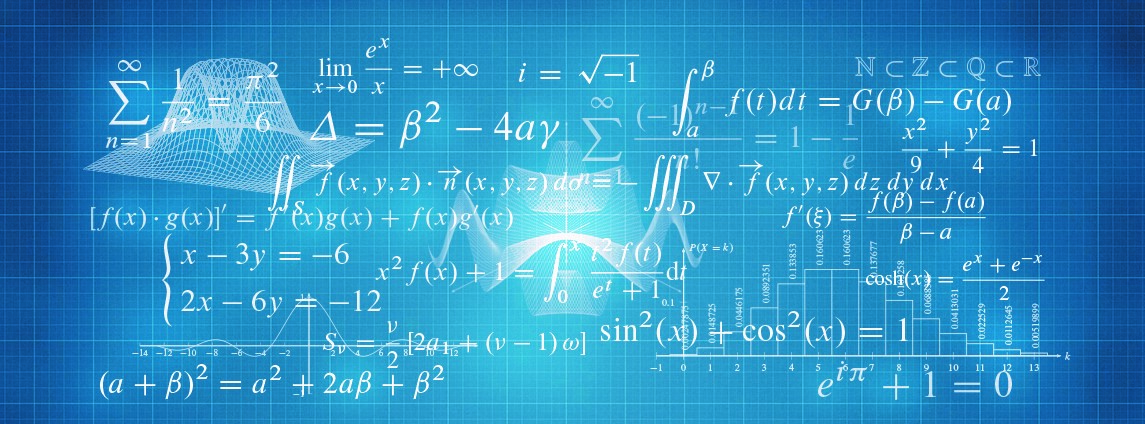
\includegraphics[width=17cm]{Kefalaio}};
\node[anchor=west,xshift=.1\paperwidth,yshift=.14\paperheight,rectangle]
{{\color{white}\fontsize{30}{20}\textbf{\textcolor{black}{\contour{white}{ΚΕΦΑΛΑΙΟ}}}}};
\node[anchor=west,xshift=.09\paperwidth,yshift=.08\paperheight,rectangle] {\fontsize{24}{20} {\color{black}{{\textcolor{black}{\contour{white}{\sc##1}}}}}};
%\fill[fill=black] (12.2,2) rectangle (14.8,4.7);
\node[anchor=west,xshift=.74\paperwidth,yshift=.11\paperheight,rectangle]
{{\color{white}\fontsize{80}{20}\textbf{\textit{\textcolor{white}{\contour{black}{\thechapter}}}}}};
\end{tikzpicture}
};
\end{tikzpicture}
}
\titlespacing*{\chapter}{0pt}{20pt}{30pt}
}
%------------------------------------------------


\usepackage[outline]{contour}
\newcommand{\regularchapter}{%
\titleformat{\chapter}[display]
{\normalfont\huge\bfseries}{\chaptertitlename\ \thechapter}{20pt}{\Huge##1}
\titlespacing*{\chapter}
{0pt}{-20pt}{40pt}
}

\apptocmd{\mainmatter}{\fancychapter}{}{}
\apptocmd{\backmatter}{\regularchapter}{}{}
\apptocmd{\frontmatter}{\regularchapter}{}{}

\titlespacing*{\section}
{0pt}{30pt}{0pt}
\usepackage{booktabs}
\usepackage{hhline}
\DeclareRobustCommand{\perthousand}{%
\ifmmode
\text{\textperthousand}%
\else
\textperthousand
\fi}


\contentsmargin{0cm}
\titlecontents{part}[-1pc]
{\addvspace{10pt}%
\bf\Large ΜΕΡΟΣ\quad }%
{}
{}
{\;\dotfill}%
%------------------------------------------
\titlecontents{chapter}[0pc]
{\addvspace{30pt}%
\begin{tikzpicture}[remember picture, overlay]%
\draw[fill=black,draw=black] (-.3,.5) rectangle (3.7,1.1); %
\pgftext[left,x=0cm,y=0.75cm]{\color{white}\sc\Large\bfseries Κεφάλαιο\ \thecontentslabel};%
\end{tikzpicture}\large\sc}%
{}
{}
{\hspace*{-2.3em}\hfill\normalsize Σελίδα \thecontentspage}%
\titlecontents{section}[2.4pc]
{\addvspace{1pt}}
{\contentslabel[\thecontentslabel]{2pc}}
{}
{\;\dotfill\;\small \thecontentspage}
[]
\titlecontents*{subsection}[4pc]
{\addvspace{-1pt}\small}
{}
{}
{\ --- \small\thecontentspage}
[ \textbullet\ ][]

\makeatletter
\renewcommand{\tableofcontents}{%
\chapter*{%
\vspace*{-20\p@}%
\begin{tikzpicture}[remember picture, overlay]%
\pgftext[right,x=12cm,y=0.2cm]{\Huge\sc\bfseries \contentsname};%
\draw[fill=black,draw=black] (9.5,-.75) rectangle (12.5,1);%
\clip (9.5,-.75) rectangle (15,1);
\pgftext[right,x=12cm,y=0.2cm]{\color{white}\Huge\bfseries \contentsname};%
\end{tikzpicture}}%
\@starttoc{toc}}
\makeatother

\usepackage[contents={},scale=1,opacity=1,color=black,angle=0]{background}

\newcommand\blfootnote[1]{%
\begingroup
\renewcommand\thefootnote{}\footnote{#1}%
\addtocounter{footnote}{-1}%
\endgroup
}
\usepackage{epstopdf}
\epstopdfsetup{update}
\usepackage{textcomp}

\titleformat{\section}
{\normalfont\Large\bf}%
{}{0em}%
{{\color{black}\titlerule[0pt]}\vskip-.2\baselineskip{\parbox[t]{\dimexpr\textwidth-2\fboxsep\relax}{\raggedright\strut\itshape{\LARGE{\thesection~#1}}\strut}}}[\vskip 0\baselineskip{\color{black}\titlerule[1pt]}]
\titlespacing*{\section}{0pt}{0pt}{30pt}

\newcommand{\methodologia}{\begin{center}
{\large \textbf{ΜΕΘΟΔΟΛΟΓΙΑ}}\\\vspace{-2mm}
\begin{tikzpicture}
\shade[left color=white, right color=black,] (-3cm,0) rectangle (0,.2mm);
\shade[left color=black, right color=white,] (0,0) rectangle (3cm,.2mm);   
\end{tikzpicture}
\end{center}}

\newcommand{\orismoi}{\begin{center}
\vspace{-3mm}{\large \textbf{\textcolor{\xrwma}{ΟΡΙΣΜΟΙ}}}\\\vspace{-2mm}
\begin{tikzpicture}
\shade[left color=white, right color=cyan!80!black,] (-3cm,0) rectangle (0,.2mm);
\shade[left color=cyan!80!black, right color=white,] (0,0) rectangle (3cm,.2mm);   
\end{tikzpicture}
\end{center}}
\newcommand{\thewrhmata}{\begin{center}
{\large \textbf{\textcolor{\xrwmath}{ΘΕΩΡΗΜΑΤΑ - ΠΟΡΙΣΜΑΤΑ - ΠΡΟΤΑΣΕΙΣ\\ΚΡΙΤΗΡΙΑ - ΙΔΙΟΤΗΤΕΣ}}}\\\vspace{-2mm}
\begin{tikzpicture}
\shade[left color=white, right color=\xrwmath,] (-5cm,0) rectangle (0,.2mm);
\shade[left color=\xrwmath, right color=white,] (0,0) rectangle (5cm,.2mm);   
\end{tikzpicture}
\end{center}}
\usepackage[labelfont={footnotesize,it,bf},font={footnotesize}]{caption}

%-------- ΠΙΝΑΚΕΣ ---------
\usepackage{booktabs}
%----------------------
%----- ΥΠΟΛΟΓΙΣΤΗΣ ----------
%\usepackage{calculator}
%----------------------------

%----- ΟΡΙΖΟΝΤΙΑ ΛΙΣΤΑ ------
\usepackage{xparse}
\newcounter{answers}
\renewcommand\theanswers{\arabic{answers}}
\ExplSyntaxOn
\NewDocumentCommand{\results}{m}
{
\seq_set_split:Nnn \l_results_a_seq {,}{#1}
\par\nobreak\noindent\setcounter{answers}{0}
\seq_map_inline:Nn \l_results_a_seq
{
\makebox[.18\linewidth][l]{\stepcounter{answers}\theanswers.~##1}\hfill
}
\par
}
\seq_new:N \l_results_a_seq
\ExplSyntaxOff
%----------------------------
%------ ΜΗΚΟΣ ΓΡΑΜΜΗΣ ΚΛΑΣΜΑΤΟΣ ---------
\DeclareRobustCommand{\frac}[3][0pt]{%
{\begingroup\hspace{#1}#2\hspace{#1}\endgroup\over\hspace{#1}#3\hspace{#1}}}
%----------------------------------------
\usepackage{microtype}
\usepackage{float}

\usepackage{caption}

%---- ΟΡΙΖΟΝΤΙΟ - ΚΑΤΑΚΟΡΥΦΟ - ΠΛΑΓΙΟ ΑΓΚΙΣΤΡΟ ------
\newcommand{\orag}[3]{\node at (#1)
{$ \overcbrace{\rule{#2mm}{0mm}}^{{\scriptsize #3}} $};}

\newcommand{\kag}[3]{\node at (#1)
{$ \undercbrace{\rule{#2mm}{0mm}}_{{\scriptsize #3}} $};}

\newcommand{\Pag}[4]{\node[rotate=#1] at (#2)
{$ \overcbrace{\rule{#3mm}{0mm}}^{{\rotatebox{-#1}{\scriptsize$#4$}}}$};}
%-----------------------------------------
\tikzstyle{pl}=[line width=0.3mm]
\tikzstyle{plm}=[line width=0.4mm]
%------- ΣΤΥΛ ΠΑΡΑΔΕΙΓΜΑΤΟΣ -------
\newcounter{paradeigma}[section]
\renewcommand{\theparadeigma}{\bf\thechapter.\arabic{paradeigma}}   
\newcommand{\Paradeigma}[1]{\refstepcounter{paradeigma}\textcolor{cyan}{\textbf{{\large Παράδειγμα\hspace{2mm}\theparadeigma\;:\;}\hspace{1mm}}} \MakeUppercase{\textbf{#1}}\\}{}
%-----------------------------------

%------- ΣΤΥΛ ΛΥΣΗΣ ------------------
\newcommand{\lysh}{{\textbf{ΛΥΣΗ}}}
%------------------------------------

%------ ΛΥΜΕΝΑ ΠΑΡΑΔΕΙΓΜΑΤΑ ΤΙΤΛΟΣ ---------
\newcommand{\Lymena}{\begin{center}
\begin{tikzpicture}
\path[left color=cyan!70!black,right color=cyan!80!black,middle color=cyan!80!white] (-7cm,-.6cm) rectangle (6.5cm,.6cm);
\node at (-.25cm,0) {\Large \textcolor{white}{\textbf{ΛΥΜΕΝΑ ΠΑΡΑΔΕΙΓΜΑΤΑ}}};  
\end{tikzpicture}
\end{center}}
%--------------------------------------

%--------- ΑΛΥΤΕΣ ΑΣΚΗΣΕΙΣ ΤΙΤΛΟΣ ----------
\newcommand{\Alyta}{\begin{center}
\begin{tikzpicture}
\path[left color=cyan!70!black,right color=cyan!80!black,middle color=cyan!80!white] (-7cm,-.6cm) rectangle (6.5cm,.6cm);
\node at (-.25cm,0) {\Large \textcolor{white}{\textbf{ΑΣΚΗΣΕΙΣ - ΠΡΟΒΛΗΜΑΤΑ}}};  
\end{tikzpicture}
\end{center}}
%--------------------------------------------
\usetikzlibrary{shadows,calc}
\usepackage{tcolorbox}
\tcbuselibrary{skins,theorems,breakable}
%---------- ΜΕΘΟΔΟΣ --------------
\newcounter{Methodos}[chapter]
\renewcommand{\theMethodos}{\thechapter.\arabic{Methodos}}
\newenvironment{Methodos}[2][\linewidth]
{\refstepcounter{Methodos}
\begin{tcolorbox}[breakable,
enhanced standard,
boxrule=0.7pt,titlerule=-.2pt,fuzzy shadow={1.5mm}{-1.5mm}{0mm}{.35mm}{black!70!white},
width=\linewidth,
title style={color=white},
overlay unbroken and first={
\path[left color=cyan!70!black,right color=cyan,draw=black]
([yshift=-\pgflinewidth]frame.north west) to ([yshift=-5pt]title.south west)[rounded corners=2pt] -- ([xshift=-#2-15pt,yshift=-5pt]title.south east) to[rounded corners=2pt] ([xshift=-#2,yshift=-\pgflinewidth]frame.north east) -- cycle;
},
fonttitle=\bfseries,
before=\par\medskip\noindent,
after=\par\medskip,
toptitle=3pt,
top=11pt,topsep at break=-5pt,
colback=white,title={\large Μέθοδος \theMethodos} : {\textcolor{black}{\MakeUppercase{#1}}}]}
{\end{tcolorbox}}
%------------------------------------------
%---------- ΛΙΣΤΕΣ ----------------------
\newlist{bhma}{enumerate}{3}
\setlist[bhma]{label=\bf\textit{\arabic*\textsuperscript{o}\;Βήμα :},leftmargin=0cm,itemindent=1.5cm,ref=\bf{\arabic*\textsuperscript{o}\;Βήμα}}
\newlist{rlist}{enumerate}{3}
\setlist[rlist]{itemsep=0mm,label=\roman*.}


%----ΣΤΥΛ ΑΣΚΗΣΗΣ ----------
\newcounter{askhsh}[chapter]
\renewcommand{\theaskhsh}{\bf{{\large{\thechapter}}.\arabic{askhsh}}}   
\newcommand{\Askhsh}{\refstepcounter{askhsh}\textcolor{\xrwma}{{\theaskhsh}\hspace{1mm}}}{}
%---------------------------

\newlist{brlist}{enumerate}{3}
\setlist[brlist]{itemsep=0mm,label=\bf\roman*.}
\newlist{tropos}{enumerate}{3}
\setlist[tropos]{label=\bf\textit{\arabic*\textsuperscript{oς}\;Τρόπος :},leftmargin=0cm,itemindent=2.3cm,ref=\bf{\arabic*\textsuperscript{oς}\;Τρόπος}}
% Αν μπει το bhma μεσα σε tropo τότε
%\begin{bhma}[leftmargin=.7cm]
\newcommand{\tss}[1]{\textsuperscript{#1}}
\newcommand{\tssL}[1]{\MakeLowercase{\textsuperscript{#1}}}
%------------------------------------------
\setlength{\parindent}{0pt}
\setlist[itemize]{itemsep=0mm}
\tkzSetUpPoint[size=7,fill=white]
\newcommand{\twocolkentro}[1]{
\twocolumn[
\begin{@twocolumnfalse}
#1
\end{@twocolumnfalse}]}
\newcommand{\bcc}[1]{
\begin{center}
{\begin{varwidth}{6.4cm}
\centering{\textbf{\textcolor{black}{#1}}}
\end{varwidth}}
\end{center}}

\DeclareMathSizes{10.95}{10.95}{7}{5}
\DeclareMathSizes{6}{6}{3.8}{2.7}
\DeclareMathSizes{8}{8}{5.1}{3.6}
\DeclareMathSizes{9}{9}{5.8}{4.1}
\DeclareMathSizes{10}{10}{6.4}{4.5}
\DeclareMathSizes{12}{12}{7.7}{5.5}
\DeclareMathSizes{14.4}{14.4}{9.2}{6.5}
\DeclareMathSizes{17.28}{17.28}{11}{7.9}
\DeclareMathSizes{20.74}{20.74}{13.3}{9.4}
\DeclareMathSizes{24.88}{24.88}{16}{11.3}

\makeatletter
\AtBeginDocument{
\check@mathfonts
\fontdimen16\textfont2=2.5pt
\fontdimen17\textfont2=2.5pt
\fontdimen14\textfont2=4.5pt
\fontdimen13\textfont2=4.5pt 
}
\makeatother



\begin{document}
\mainmatter
\pagestyle{fancy}
\chapter{Τριγωνομετρία}
\section{Τριγωνομετρικοί Αριθμοί}
\orismoi
\Orismos{Τριγωνομετρικοί αριθμοί}
Έστω $ AB\varGamma $ ένα ορθογώνιο τρίγωνο, με $ A=90\degree $ τότε οι τριγωνομετρικοί αριθμοί των οξείων γωνιών του τριγώνου ορίζονται ως εξής :\\
\wrapr{-11mm}{7}{3.5cm}{0mm}{
\begin{tikzpicture}[scale=.8]
\tkzDefPoint(0,0){A}
\tkzDefPoint(3,0){B}
\tkzDefPoint(0,3.5){C}
\tkzMarkAngle[fill=\xrwma!50,size=.5](C,B,A)
\tkzMarkRightAngle[size=.3](B,A,C)
\tkzDrawPolygon[pl](A,B,C)
\tkzText(2.2,.2){$ \omega $}
\tkzLabelPoint[left](A){$ A $}
\tkzLabelPoint[right](B){$ B $}
\tkzLabelPoint[left](C){$ \varGamma $}
\tkzDrawPoints[size=7,fill=white](A,B,C)
\end{tikzpicture}\captionof{figure}{Τριγωνομετρικοί αριθμοι οξείας γωνίας}}{
\begin{enumerate}[itemsep=0mm,label=\bf\arabic*.]
\item \textbf{Ημίτονο}\\
Ημίτονο μιας οξέιας γωνίας ενός ορθογωνίου τριγώνου ονομάζεται ο λόγος της απέναντι κάθετης πλευράς προς την υποτείνουσα.
\[ \textrm{Ημίτονο}=\frac{\textrm{Απέναντι Κάθετη}}{\textrm{Υποτείνουσα}}\;\;,\;\;\hm{\omega}=\frac{A\varGamma}{B\varGamma} \]
\item \textbf{Συνημίτονο}\\
Συνημίτονο μιας οξέιας γωνίας ενός ορθογωνίου τριγώνου ονομάζεται ο λόγος της προσκείμενης κάθετης πλευράς προς την υποτείνουσα.
\end{enumerate}
\[ \textrm{Συνημίτονο}=\frac{\textrm{Προσκείμενη Κάθετη}}{\textrm{Υποτείνουσα}}\;\;,\;\;\syn{\omega}=\frac{AB}{B\varGamma} \]}

\begin{enumerate}[itemsep=0mm,label=\bf\arabic*.,start=3]
\item \textbf{Εφαπτομένη}\\
Εφαπτομένη μιας οξείας γωνίας ενός ορθογωνίου τριγώνου ονομάζεται ο λόγος της απέναντι κάθετης πλευράς προς την προσκείμενη κάθετη.
\[ \textrm{Εφαπτομένη}=\frac{\textrm{Απέναντι Κάθετη}}{\textrm{Προσκείμενη Κάθετη}}\;\;,\;\;\ef{\omega}=\frac{A\varGamma}{AB} \]
\item \textbf{Συνεφαπτομένη}\\
Συνεφαπτομένη μιας οξείας γωνίας ενός ορθογωνίου τριγώνου ονομάζεται ο λόγος της προσκείμενης κάθετης πλευράς προς την απέναντι κάθετη.
\[ \textrm{Συνεφαπτομένη}=\frac{\textrm{Προσκείμενη Κάθετη}}{\textrm{Απέναντι Κάθετη}}\;\;,\;\;\syf{\omega}=\frac{AB}{A\varGamma} \]
\end{enumerate}
\Orismos{τριγ. αρ. γωνιασ σε συστημα συντεταγμενων}
Έστω $ Oxy $ ένα ορθογώνιο σύστημα συντεταγμένων και $ M(x,y) $ ένα σημείο του. Ενώνοντας το σημείο $ M $ με την αρχή των αξόνων, το ευθύγραμμο τμήμα που προκύπτει δημιουργεί μια γωνία $ \omega $ με το θετικό οριζόντιο ημιάξονα $ Ox $.
Το μήκος του ευθύγραμμου τμήματος $ OM $ είναι :
\[ OM=\rho=\sqrt{x^2+y^2} \]
Οι τριγωνομετρικοί αριθμοί της γωνίας $ x\hat{O}y $ ορίζονται με τη βοήθεια των συντεταγμένων του σημείου και είναι\\
\wrapr{-11mm}{8}{4.5cm}{0mm}{
\begin{tikzpicture}[y=.8cm,x=.9cm]
\draw[draw=black,fill=\xrwma!50] (0,0) -- (.5,0) arc (0:40:.5) -- cycle;
\draw[-latex]  (-.4,0)  -- coordinate (x axis mid) (4,0) node[right,fill=white] {{\footnotesize $ x $}};
\draw[-latex] (0,-.4) -- (0,3.5) node[above,fill=white] {{\footnotesize $ y $}};
\draw (3,.1) -- (3,-.1) node[anchor=north] {\scriptsize $ x $};
\draw (.1,2.5) -- (-.1,2.5) node[anchor=east] {\scriptsize $ y $};
\draw[dashed] (3,0) -- (3,2.5) -- (0,2.5);
\tkzDefPoint(0,0){O}
\tkzDefPoint(3,2.5){M}
\tkzDefPoint(3,0){A}
\tkzDefPoint(0,2.5){B}
\tkzDrawSegment(O,M)
\tkzDrawPoint[size=7,fill=white](M)
\tkzDrawPoint[size=7,fill=white](A)
\tkzDrawPoint[size=7,fill=white](B)
\tkzLabelPoint[below left](O){$ O $}
\tkzLabelPoint[above](M){{\footnotesize $ M(x,y) $}}
\tkzLabelPoint[above right](A){{\footnotesize $ A(x,0) $}}
\tkzLabelPoint[above right](B){{\footnotesize $ B(0,y) $}}
\tkzText(1.5,-.4){$ \undercbrace{\rule{23mm}{0mm}}_{{\scriptsize x}} $}
\tkzText(-.3,1.25){{{\scriptsize $ y $}}$\LEFTRIGHT\{.{ \rule{0pt}{20mm} } $}
\tkzText[fill=white,inner sep=.2mm](2.7,1){{\footnotesize $ \rho=\sqrt{x^2+y^2} $}}
\tkzText(.7,.2){{\footnotesize $ \omega $}}
\end{tikzpicture}\captionof{figure}{Τριγωνομετρικοί αριθμοί σε σύστημα συντεταγμένων.}}{
\begin{enumerate}[itemsep=0mm,label=\bf\arabic*.]
\item \textbf{Ημίτονο}\\
Ημίτονο της γωνίας  ονομάζεται ο λόγος της τεταγμένης του σημείου προς την απόσταση του από την αρχή των αξόνων.
\[ \hm{\omega}=\frac{AM}{OM}=\frac{y}{\rho} \]
\item \textbf{Συνημίτονο}\\
Συνημίτονο της γωνίας  ονομάζεται ο λόγος της τετμημένης του σημείου προς την απόσταση του από την αρχή των αξόνων.
\[ \syn{\omega}=\frac{BM}{OM}=\frac{x}{\rho} \]
\end{enumerate}

\begin{enumerate}[itemsep=0mm,label=\bf\arabic*.,start=3]
\item \textbf{Εφαπτομένη}\\
Εφαπτομένη της γωνίας ονομάζεται ο λόγος της τεταγμένης του σημείου προς την τετμημένη του.
\[ \ef{\omega}=\frac{AM}{BM}=\frac{y}{x}\;\;,\;\;x\neq0 \]
\item \textbf{Συνεφαπτομένη}\\
Συνεφαπτομένη της γωνίας  ονομάζεται ο λόγος της τετμημένης του σημείου προς την τεταγμένη του.
\[ \syf{\omega}=\frac{BM}{AM}=\frac{x}{y}\;\;.\;\;y\neq0 \]
\end{enumerate}}
\Orismos{μοναδεσ μετρησησ γωνιων - τοξων}
Μονάδες μέτρησης γωνιών - τόξων λέγονται οι γωνίες ή τα τόξα αντίστοιχα με τα οποία μετράμε το μέτρο (άνοιγμα) των πλευρών μιας γωνίας ή αντίστοιχα το μέτρο ενός τόξου.
Οι βασικές μονάδες μέτρησης για τη μέτρηση γωνιών ή τόξων είναι :
\begin{enumerate}[itemsep=0mm,label=\bf\arabic*.]
\item \textbf{Μοίρα}\\
Μοίρα ονομάζεται το τόξο το οποίο είναι ίσο με το $ \frac{1}{360} $ του τόξου ενός κύκλου.
Ισοδύναμα είναι η γωνία η οποία αν γίνει επίκεντρη σε κύκλο, βαίνει σε τόξο ίσο με το $ \frac{1}{360} $ του κύκλου.
\begin{itemize}[itemsep=0mm]
\item Συμβολίζεται με $ 1\degree $.
\item Μια μοίρα χωρίζεται σε 60 πρώτα λεπτά $ (60') $ και κάθε λεπτό σε 60 δεύτερα λεπτά $ (60'') $.
\end{itemize}
\item \textbf{Ακτίνιο}\\
Ακτίνιο ονομάζεται το τόξο ενός κύκλου του οποίου το μήκος είναι ίσο με την ακτίνα του κύκλου. Ορίζεται και ως η γωνία που αν γίνει επίκεντρη, βαίνει σε τόξο με μήκος ίσο με την ακτίνα του κύκλου.
Συμβολίζεται με $ 1rad $.
\end{enumerate}

\begin{center}
\begin{tabular}{c||>{\centering\arraybackslash}m{.8cm}>{\centering\arraybackslash}m{.8cm}>{\centering\arraybackslash}m{.8cm}>{\centering\arraybackslash}m{.8cm}>{\centering\arraybackslash}m{.8cm}>{\centering\arraybackslash}m{.8cm}>{\centering\arraybackslash}m{.8cm}>{\centering\arraybackslash}m{.8cm}>{\centering\arraybackslash}m{.8cm}}
\hline  \multicolumn{10}{c}{\textbf{Βασικές Γωνίες}} \rule[-2ex]{0pt}{5ex}  \\ 
\hhline{==========} \rule[-2ex]{0pt}{5ex} \textbf{Μοίρες} & $ 0\degree $ & $ 30\degree $ & $ 45\degree $ & $ 60\degree $ & $ 90\degree $ & $ 120\degree $ & $ 135\degree $ & $ 150\degree $ & $ 180\degree $ \\ 
\rule[-2ex]{0pt}{4ex} \textbf{Ακτίνια} & $ 0 $ & $ \frac{\pi}{6} $ & $ \frac{\pi}{4} $ & $ \frac{\pi}{3} $ & $ \frac{\pi}{2} $ & $ \frac{2\pi}{3} $ & $ \frac{3\pi}{4} $ & $ \frac{5\pi}{6} $ & $ \pi $ \\ 
\hline \rule[-2ex]{0pt}{5.5ex} \textbf{Σχήμα} & \begin{tikzpicture}
\fill[fill=\xrwma!50] (0,0) -- (.3,0) arc (0:0:.3) -- cycle;
\draw (-.35,0) -- (.35,0);
\draw (0,-.35) -- (0,.35);
\draw (0,0) circle (.3);
\coordinate (A) at (0:.3);
\draw (0,0) -- (A);
\end{tikzpicture} & \begin{tikzpicture}
\fill[fill=\xrwma!50] (0,0) -- (.3,0) arc (0:30:.3) -- cycle;
\draw (-.35,0) -- (.35,0);
\draw (0,-.35) -- (0,.35);
\draw (0,0) circle (.3);
\coordinate (A) at (30:.3);
\draw (0,0) -- (A);
\end{tikzpicture} & \begin{tikzpicture}
\fill[fill=\xrwma!50] (0,0) -- (.3,0) arc (0:45:.3) -- cycle;
\draw (-.35,0) -- (.35,0);
\draw (0,-.35) -- (0,.35);
\draw (0,0) circle (.3);
\coordinate (A) at (45:.3);
\draw (0,0) -- (A);
\end{tikzpicture} & \begin{tikzpicture}
\fill[fill=\xrwma!50] (0,0) -- (.3,0) arc (0:60:.3) -- cycle;
\draw (-.35,0) -- (.35,0);
\draw (0,-.35) -- (0,.35);
\draw (0,0) circle (.3);
\coordinate (A) at (60:.3);
\draw (0,0) -- (A);
\end{tikzpicture} & \begin{tikzpicture}
\fill[fill=\xrwma!50] (0,0) -- (.3,0) arc (0:90:.3) -- cycle;
\draw (-.35,0) -- (.35,0);
\draw (0,-.35) -- (0,.35);
\draw (0,0) circle (.3);
\coordinate (A) at (90:.3);
\draw (0,0) -- (A);
\end{tikzpicture} & \begin{tikzpicture}
\fill[fill=\xrwma!50] (0,0) -- (.3,0) arc (0:120:.3) -- cycle;
\draw (-.35,0) -- (.35,0);
\draw (0,-.35) -- (0,.35);
\draw (0,0) circle (.3);
\coordinate (A) at (120:.3);
\draw (0,0) -- (A);
\end{tikzpicture} & \begin{tikzpicture}
\fill[fill=\xrwma!50] (0,0) -- (.3,0) arc (0:135:.3) -- cycle;
\draw (-.35,0) -- (.35,0);
\draw (0,-.35) -- (0,.35);
\draw (0,0) circle (.3);
\coordinate (A) at (135:.3);
\draw (0,0) -- (A);
\end{tikzpicture} & \begin{tikzpicture}
\fill[fill=\xrwma!50] (0,0) -- (.3,0) arc (0:150:.3) -- cycle;
\draw (-.35,0) -- (.35,0);
\draw (0,-.35) -- (0,.35);
\draw (0,0) circle (.3);
\coordinate (A) at (150:.3);
\draw (0,0) -- (A);
\end{tikzpicture} & \begin{tikzpicture}
\fill[fill=\xrwma!50] (0,0) -- (.3,0) arc (0:180:.3) -- cycle;
\draw (-.35,0) -- (.35,0);
\draw (0,-.35) -- (0,.35);
\draw (0,0) circle (.3);
\coordinate (A) at (180:.3);
\draw (0,0) -- (A);
\end{tikzpicture} \\ 
\hline \rule[-2ex]{0pt}{5ex} $ \hm{\omega} $ & $ 0 $ & $ \frac{1}{2} $ & $ \frac{\sqrt{2}}{2} $ & $ \frac{\sqrt{3}}{2} $ & $ 1 $ & $ \frac{\sqrt{3}}{2} $ & $ \frac{\sqrt{2}}{2} $ & $ \frac{1}{2} $ & $ 0 $ \\ 
\rule[-2ex]{0pt}{4ex} $ \syn{\omega} $ & $ 1 $ & $ \frac{\sqrt{3}}{2} $ & $ \frac{\sqrt{2}}{2} $ & $ \frac{1}{2} $ & $ 0 $ & $ -\frac{1}{2} $ & $ -\frac{\sqrt{2}}{2} $ & $ -\frac{\sqrt{3}}{2} $ & $ -1 $ \\ 
\rule[-2ex]{0pt}{4ex} $ \ef{\omega} $ & $ 0 $ & $ \frac{\sqrt{3}}{3} $ & $ 1 $ & $ \sqrt{3} $ & \begin{minipage}{.8cm}
\begin{center}
{\scriptsize Δεν\\\vspace{-1mm}ορίζεται}
\end{center}
\end{minipage} & $ -\sqrt{3} $ & $ -1 $ & $ -\frac{\sqrt{3}}{3} $ & $ 0 $ \\
\rule[-2ex]{0pt}{4ex} $ \syf{\omega} $ & \begin{minipage}{.8cm}
\begin{center}
{\scriptsize Δεν\\\vspace{-1mm}ορίζεται}
\end{center}
\end{minipage} & $ \sqrt{3} $ & $ 1 $ & $ \frac{\sqrt{3}}{3} $ & $ 0 $ & $ -\frac{\sqrt{3}}{3} $ & $ -1 $ & $ -\sqrt{3} $ & \begin{minipage}{.8cm}
\begin{center}
{\scriptsize Δεν\\\vspace{-1mm}ορίζεται}
\end{center}
\end{minipage} \\ 
\hline 
\end{tabular}\captionof{table}{Τριγωνομετρικοί αριθμοί βασικών γωνιών}
\end{center}
\Orismos{τριγωνομετρικοσ κυκλοσ}
Τριγωνομετρικός κύκλος ονομάζεται ο κύκλος με ακτίνα ίση με τη μονάδα και κέντρο την αρχή των αξόνων ενός ορθογωνίου συστήματος συντεταγμένων, στους άξονες του οποίου παίρνουν τιμές οι τριγωνομετρικοί αριθμοί των γωνιών.
\begin{center}
\begin{tabular}{p{6.5cm}p{6.5cm}}
\multicolumn{2}{c}{{\Large \textbf{Τριγωνομετρικός Κύκλος}}}\\
\begin{tikzpicture}[>=latex,scale=2]
\fill[fill=\xrwma!50] (0,0) -- (.2,0) arc (0:60:.2) -- cycle;
%axis
\draw[->] (-1.2,0) -- coordinate (x axis mid) (1.5,0) node[right,fill=white] {{\footnotesize $ x $}};
\foreach \x in {-1,-0.8,-0.6,-0.4,-0.2,0,0.2,0.4,0.6,0.8,1}
\draw (\x,.5pt) -- (\x,-.5pt)
node[anchor=north] {{\tiny \x}};
\foreach \y in {-1,-0.8,-0.6,-0.4,-0.2,0,0.2,0.4,0.6,0.8,1}
\draw (.5pt,\y) -- (-.5pt,\y)
node[anchor=east] {{\tiny \y}};
\draw[->] (0,-1.2) -- (0,1.5) node[above,fill=white] {{\footnotesize $ y $}};
\draw[-] (1,-1.2) -- (1,1.8);
\draw[-] (-1.2,1) -- (1.2,1);
\draw[-,thick] (0,1) -- (1.732/3,1);
\draw[-,thick] (1,0) -- (1,1.732);
\draw[-,dashed] (-.7,-1.732*0.7) -- (1,1.732);
\draw circle (1);
\coordinate (A) at (60:1);
\tkzDefPoint(0,0){O}
\tkzDefPoint(cos(pi/3),0){B}
\tkzDefPoint(0,sin(pi/3)){C}
\tkzDefPoint(1,tan(pi/3)){D}
\tkzDefPoint(cot(pi/3),1){E}
\tkzDefPoint(1,0){F}
\tkzDefPoint(0,1){G}
\tkzDrawSegment(O,A)
\tkzDrawSegments[thin,dashed](A,B A,C)
\tkzText(0,1.75){{\scriptsize Άξονας Ημιτόνων}}
\tkzText(1.6,-.12){{\scriptsize Άξονας}}
\tkzText(1.6,-.23){{\scriptsize Συνημιτόνων}}
\tkzText(-1,1.22){{\scriptsize Άξονας}}
\tkzText(-.75,1.1){{\scriptsize Συνεφαπτομένων}}
\tkzText(1.23,-.87){{\scriptsize Άξονας}}
\tkzText(1.42,-1){{\scriptsize Εφαπτομένων}}
\tkzText(-.5,-1.1){{\scriptsize $ \delta $}}
\tkzDrawSegment[thick](O,B)
\tkzDrawSegment[thick](O,C)
\tkzDrawPoints[size=7,fill=white](O,A,B,C,D,E,F,G)
\tkzText(-.4,.43){{{\scriptsize \textrm{ημ}$ \omega $}}$\LEFTRIGHT\{.{ \rule{0pt}{18mm} } $}
\tkzText(.25,-.25){$ \undercbrace{\rule{9mm}{0mm}}_{{\scriptsize \textrm{συν}\omega}} $}
\tkzText(1.2,.87){$\LEFTRIGHT.\}{ \rule{0pt}{33mm} } ${{\scriptsize \textrm{εφ}$ \omega $}}}
\tkzText(.3,1.12){$ \overcbrace{\rule{10mm}{0mm}}^{{\scriptsize \textrm{σφ}\omega}} $}
\tkzText(.25,.15){$ \omega $}
\tkzLabelPoint[below left,xshift=.5mm,yshift=.5mm](O){{\tiny $ O $}}
\tkzLabelPoint[above=1mm,right](A){{\tiny $ M $}}
\tkzLabelPoint[above right](B){{\tiny $ M_1 $}}
\tkzLabelPoint[above=1mm, left](C){{\tiny $ M_2 $}}
\tkzLabelPoint[left](D){{\tiny $ K $}}
\tkzLabelPoint[above](E){{\tiny $ \varLambda $}}
\tkzLabelPoint[below right](F){{\tiny $ A $}}
\tkzLabelPoint[above left](G){{\tiny $ B $}}
\draw [->] (.984*.9,.173*.9) arc (10:45:.9);
\draw [->] (.984*.9,-.173*.9) arc (-10:-45:.9);
\tkzText(.72,.35){$ + $}
\tkzText(.72,-.35){$ - $}
\tkzText(.35,.45){$ \rho $}
\tkzText(-1,.9){{\scriptsize $ \varepsilon_2 $}}
\tkzText(.9,-1){{\scriptsize $ \varepsilon_1 $}}
\end{tikzpicture}\captionof{figure}{Τριγωνομετρικός κύκλος} & \begin{tikzpicture}[>=latex,scale=2]
\fill[fill=\xrwma!50] (0,0) -- (.2,0) arc (0:45:.2) -- cycle;
%axis
\draw[->] (-1.2,0) -- (1.5,0) node[right,fill=white] {{\footnotesize $ x $}};
\draw[->] (0,-1.2) -- (0,1.5) node[above,fill=white] {{\footnotesize $ y $}};

\foreach \gwnia/\xtext in {
30/\frac{\pi}{6},
45/\frac{\pi}{4},
60/\frac{\pi}{3},
90/\frac{\pi}{2},
120/\frac{2\pi}{3},
135/\frac{3\pi}{4},
150/\frac{5\pi}{6},
180/\pi,
210/\frac{7\pi}{6},
240/\frac{4\pi}{3},
270/\frac{3\pi}{2},
300/\frac{5\pi}{3},
330/\frac{11\pi}{6},
360/2\pi}
\draw (\gwnia:0.85cm) node {{\scriptsize $\xtext$}};
\foreach \gwnia/\xtext in {
90/\frac{\pi}{2},
180/\pi,
270/\frac{3\pi}{2},
360/2\pi}
\draw (\gwnia:0.85cm) node[fill=white] {{\scriptsize $\xtext$}};
\tkzDefPoint(0,0){O}
\coordinate (A) at (45:1);
\tkzDrawSegment(O,A)
\draw circle (1);
\foreach \gwnia in {0,30,45,60,90,120,135,150,180,210,240,270,300,330}{
\coordinate (P) at (\gwnia:1);
\draw (\gwnia:1.22cm) node[fill=white,inner sep=0.1mm] {{\scriptsize $\gwnia^\circ$}};
\draw[draw=black,fill=white] (P) circle (.7pt);};
\tkzText(.25,.1){$ \omega $}
\end{tikzpicture}\captionof{figure}{Βασικές γωνίες}
\end{tabular}
\end{center}
\begin{itemize}[itemsep=0mm]
\item Κάθε γωνία $ \omega $ έχει πλευρές, τον θετικό ημιάξονα $ Ox $ και την ακτίνα $ \rho $ του κύκλου, μετρώντας τη γωνία αυτή αριστερόστροφα, φορά που ορίζεται ως \textbf{θετική}.
\item Ο οριζόντιος άξονας $ x'x $ είναι ο άξονας συνημιτόνων ενώ ο κατακόρυφος $ y'y $ ο άξονας ημιτόνων.
\item Κάθε σημείο $ M $ του κύκλου έχει συντεταγμένες $ M(\syn{\omega},\hm{\omega}) $.
\item Η τετμημέμη του σημείου είναι ίση με το συνημίτονο της γωνίας, ενώ η τεταγμένη ίση με το ημίτονο της.
\[ x=\syn{\omega}\;\;,\;\;y=\hm{\omega} \]
\item Η εφαπτόμενη ευθεία στον κύκλο στο σημείο $ A(1,0) $ είναι ο \textbf{άξονας των εφαπτομένων}. Η εφαπτομένη της γωνίας $ \omega $ είναι η τεταγμένη του σημείου τομής της ευθείας $ \varepsilon_1 $ με το φορέα $ \delta $ της ακτίνας.
\[ y_{\!_K}=\ef{\omega} \]
\item Η εφαπτόμενη ευθεία στον κύκλο στο σημείο $ B(0,1) $ είναι ο \textbf{άξονας των συνεφαπτομένων}. Η συνεφαπτομένη της γωνίας $ \omega $ είναι η τετμημένη του σημείου τομής της ευθείας $ \varepsilon_2 $ με το φορέα $ \delta $ της ακτίνας.
\[ x_{\!_K}=\syf{\omega} \]	
\end{itemize}
Πιο κάτω βλέπουμε τα τέσσερα τεταρτημόρια στα οποία χωρίσουν οι άξονες το επίπεδο και τον τριγωνομετρικό κύκλο καθώς και το πρόσημο των τριγωνομετρικών αριθμών των γωνιών σε κάθε τεταρτημόριο.
\begin{center}
\begin{minipage}[m]{6cm}
\centering
\begin{tabular}{c|cccc}
\hline \textbf{Τεταρτημόριο} & \textbf{{$ \mathbold{\hm{\omega}} $}} & \textbf{{$ \mathbold{\syn{\omega}} $}} & \textbf{{$ \mathbold{\ef{\omega}} $}} & \textbf{{$ \mathbold{\syf{\omega}} $}} \rule[-2ex]{0pt}{5ex}\\ 
\hhline{=====} \rule[-2ex]{0pt}{5ex} \textbf{1\tss{o} Τεταρτημόριο} & $ + $ & $ + $ & $ + $ & $ + $ \\ 
\rule[-2ex]{0pt}{5ex} \textbf{2\tss{o} Τεταρτημόριο} & $ + $ & $ - $ & $ - $ & $ - $ \\ 
\rule[-2ex]{0pt}{5ex} \textbf{3\tss{o} Τεταρτημόριο} & $ - $ & $ - $ & $ + $ & $ + $ \\ 
\rule[-2ex]{0pt}{5ex} \textbf{4\tss{o} Τεταρτημόριο} & $ - $ & $ + $ & $ - $ & $ - $ \\ 
\hline 
\end{tabular}\captionof{table}{Πρόσημα τριγωνομετρικών αριθμών}
\end{minipage}\hspace{2.cm}
\begin{minipage}[m]{5cm}
\centering
\begin{tikzpicture}[scale=1.8]
\draw[-latex] (-1.2,0) -- (1.2,0) node[right,fill=white] {{\footnotesize $ x $}};
\draw[-latex] (0,-1.2) -- (0,1.2) node[above,fill=white] {{\footnotesize $ y $}};
\tkzDefPoint(0,0){O}
\draw circle (1);
\tkzLabelPoint[below left,xshift=.5mm,yshift=.5mm](O){$ O $}
\node at (0.4,0.5) {{\scriptsize 1\textsuperscript{o} Τετ.}};
\node at (0.4,-0.5) {{\scriptsize 4\textsuperscript{o} Τετ.}};
\node at (-0.4,-0.5) {{\scriptsize 3\textsuperscript{o} Τετ.}};
\node at (-0.4,0.5) {{\scriptsize 2\textsuperscript{o} Τετ.}};
\node at (0.4,0.3) {{\scriptsize $ (+,+) $}};
\node at (-0.4,0.3) {{\scriptsize $ (-,+) $}};
\node at (-0.4,-0.3) {{\scriptsize $ (-,-) $}};
\node at (0.4,-0.3) {{\scriptsize $ (+,-) $}};
\end{tikzpicture}\captionof{figure}{Τεταρτημόρια και πρόσημα τεταρτημορίων τριγωνομετρικού κύκλου.}
\end{minipage}
\end{center}
\thewrhmata
\Thewrhma{Όρια τριγωνομετρικών αριθμών}
To ημίτονο και το συνημίτονο οποιασδήποτε γωνίας $ \omega $ παίρνει τιμές από $-1$ μέχρι $ 1 $. Οι παρακάτω σχέσεις είναι ισοδύναμες :
\begin{multicols}{2}
\begin{rlist}
\item  $ -1\leq\hm{\omega}\leq1\;\;,\;\;-1\leq\syn{\omega}\leq1 $
\item $ |\hm{\omega}|\leq1\ ,\ |\syn{\omega}|\leq1 $
\end{rlist}
\end{multicols}
\Thewrhma{Τρ. Αριθμοί γωνιών μεγαλύτερων του κύκλου}
Οι τριγωνομετρικοί αριθμοί μιας γωνίας $ \omega $ της οποίας το μέτρο είναι μικρότερο του ενός κύκλου είναι ίσοι με τους τριγωνομετρικούς αριθμούς της γωνίας που θα προκύψει εαν στρέψουμε την $ \omega $ κατά πολλαπλάσια του κύκλου.
\begin{center}
$ \begin{array}{cc}
\hm{\left( 360\degree\cdot \kappa+\omega\right) }=\hm{\omega} & \syn{\left( 360\degree\cdot \kappa+\omega\right) }=\syn{\omega} \\ 
\ef{\left( 360\degree\cdot \kappa+\omega\right) }=\ef{\omega} & \syf{\left( 360\degree\cdot \kappa+\omega\right) }=\syf{\omega}
\end{array} $
\end{center}
ή ισοδύναμα με τη βοήθεια ακτινίων
\begin{center}
$ \begin{array}{cc}
\hm{\left( 2\kappa\pi+\omega\right) }=\hm{\omega} & \syn{\left( 2\kappa\pi+\omega\right) }=\syn{\omega} \\ 
\ef{\left( 2\kappa\pi+\omega\right) }=\ef{\omega} & \syf{\left( 2\kappa\pi+\omega\right) }=\syf{\omega}
\end{array} $
\end{center}
\Thewrhma{Μετατροπή μοιρών σε ακτίνια}
Αν $ \mu $ είναι το μέτρο μιας γωνίας σε μοίρες και $ a $ το μέτρο της ίδιας γωνίας σε ακτίνια, η σχέση που τα συνδέει και με την οποία μπορούμε να μετατρέψουμε το μέτρο μιας γωνίας από μοίρες σε ακτίνια και αντίστροφα είναι :
\[ \frac{\mu}{180\degree}=\frac{a}{\pi} \]
\newpage
\noindent
\Alyta
\begin{multicols}{2}
\Askhsh \textbf{Μετατροπή μοιρών σε ακτίνια}\\
Οι παρακάτω γωνίες οι οποίες είναι δοσμένες σε μοίρες να εκφραστούν σε ακτίνια (rad).
\begin{multicols}{3}
\begin{rlist}
\item $ 30\degree $
\item $ 60\degree $
\item $ 45\degree $
\item $ 120\degree $
\item $ 150\degree $
\item $ 300\degree $
\item $ 270\degree $
\item $ 240\degree $
\item $ 330\degree $
\item $ 400\degree $
\item $ 480\degree $
\item $ 1200\degree $
\end{rlist}
\end{multicols}
\Askhsh \textbf{Μετατροπή ακτινίων σε μοίρες}\\
Οι παρακάτω γωνίες οι οποίες είναι δοσμένες σε ακτίνια να εκφραστούν σε μοίρες.
\begin{multicols}{3}
\begin{rlist}
\item $ \frac{\pi}{4} $
\item $ \frac{2\pi}{3} $
\item $ \frac{\pi}{6} $
\item $ \frac{3\pi}{4} $
\item $ \frac{2\pi}{5} $
\item $ \pi $
\item $ \frac{3\pi}{2} $
\item $ \frac{4\pi}{5} $
\item $ 24\pi $
\item $ \frac{35\pi}{3} $
\item $ \frac{105\pi}{4} $
\item $ 400\pi $
\end{rlist}
\end{multicols}
\Askhsh \textbf{Τριγωνομετρικοί αριθμοί}\\
Να υπολογίσετε τους τριγωνομετρικούς αριθμούς των παρακάτω γωνιών.
\begin{multicols}{3}
\begin{rlist}
\item $ 390\degree $
\item $ 450\degree $
\item $ 780\degree $
\item $ 1260\degree $
\item $ 1125\degree $
\item $ 1845\degree $
\end{rlist}
\end{multicols}
\Askhsh \textbf{Τρ. αριθμοί γωνίας σε καρτεσιανό σύστημα}\\
Να υπολογίσετε τους τριγωνομετρικούς αριθμούς της γωνίας $ x\hat{O}M $ η οποία σχηματίζεται μέσα σε ένα ορθοκανονικό σύστημα συντεταγμένων $ xOy $ για καθένα από τα παρακάτω σημεία $ M $.
\begin{multicols}{2}
\begin{rlist}[leftmargin=4mm]
\item $ M(3,4) $
\item $ M(5,12) $
\item $ M(-8,15) $
\item $ M(6,-8) $
\item $ M(-4,-3) $
\item $ M(12,-9) $
\end{rlist}
\end{multicols}
\Askhsh \textbf{Τριγωνομετρικοί αριθμοί σε τρίγωνο}\\
Να υπολογίσετε τους τριγωνομετρικούς αριθμούς της γωνίας $ \omega $ σε καθένα από τα παρακάτω ορθογώνια τρίγωνα.

\Askhsh \textbf{Τρ. αριθμοί βασικών γωνιών}\\
Να υπολογίσετε τις παρακάτω αριθμητικές παραστάσεις.
\begin{multicols}{2}
\begin{rlist}[leftmargin=4mm]
\item $ \hm{30\degree}\cdot\hm{60\degree} $
\item $ \hm^2{40\degree}-2\syn{60\degree} $
\item $ \ef{45\degree}+2\syn^2{30\degree} $
\item $ \syf^2{60\degree}-\hm^2{60\degree} $
\end{rlist}
\end{multicols}
\end{multicols}
\section{Τριγωνομετρικές Ταυτότητες}
\orismoi
\Orismos{Ταυτότητα}
Ταυτότητα ονομάζεται κάθε ισότητα η οποία περιέχει μεταβλητές και αληθεύει για κάθε τιμή των μεταβλητών. Συγκεκριμένα, οι ταυτότητες οι οποίες περιέχουν τριγωνομετρικούς αριθμούς θα ονομάζονται τριγωνομετρικές ταυτότητες.
\thewrhmata
\Thewrhma{βασικεσ τριγωνομετρικεσ ταυτοτητεσ}
Για οποιαδήποτε γωνία $ \omega $ ισχύουν οι παρακάτω βασικές τριγωνομετρικές ταυτότητες :
\begin{multicols}{3}
\begin{enumerate}[itemsep=0mm]
\item $ \hm^2{\omega}+\syn^2{\omega}=1 $
\item $ \ef{\omega}={\dfrac{\hm{\omega}}{\syn{\omega}}} $
\item $ \syf{\omega}={\dfrac{\syn{\omega}}{\hm{\omega}}} $
\item $ \ef{\omega}\cdot\syf{\omega}=1 $
\item $ \syn^2{\omega}=\dfrac{1}{1+\ef^2{\omega}} $
\item $ \hm^2{\omega}=\dfrac{\ef^2{\omega}}{1+\ef^2{\omega}} $
\end{enumerate}
\end{multicols}
\section{Αναγωγή στο 1ο τεταρτημόριο}
\thewrhmata
\Thewrhma{αναγωγη στο 1\textsuperscript{\MakeLowercase{o}} τεταρτημοριο}\label{th:an_tet}
Οι τριγωνομετρικοί αριθμοί γωνιών που καταλήγουν στο 2\tss{ο}, 3\tss{ο} ή 4\tss{ο} ανάγωνται σε τριγωνομετρικούς αριθμούς γωνιών του 1\textsuperscript{ου} τεταρτημορίου σύμφωνα με τους παρακάτω τύπους.
\begin{enumerate}[itemsep=0mm,label=\bf\arabic*.]
\item \textbf{Παραπληρωματικές γωνίες (2\textsuperscript{ο} τεταρτημόριο)}\\
Γωνίες που καταλήγουν στο 2\tss{ο} τεταρτημόριο μπορούν να γραφτούν ως παραπληρωματικές γωνιών του 1\tss{ου} τεταρτημορίου. Εαν $ \omega $ είναι μια γωνία του 1\textsuperscript{ου} τεταρτημορίου τότε η παραπληρωματική της θα είναι της μορφής $ 180\degree-\omega $. Οι σχέσεις μεταξύ των τριγωνομετρικών τους αριθμών φαίνονται παρακάτω :\\
\begin{minipage}{\linewidth}\mbox{}\\
\vspace{-1.1cm}
\begin{WrapText1}{7}{6cm}
\begin{tikzpicture}[>=latex,scale=2]
\clip (-1.5,-.3) rectangle (1.4,1.4);
\draw[fill=\xrwma!10] (0,0) -- (.2,0) arc (0:40:.2) -- cycle;
\draw[fill=\xrwma!30] (0,0) -- (.15,0) arc (0:140:.15) -- cycle;
%axis
\draw[->] (-1.2,0) -- (1.2,0) node[right,fill=white] {{\footnotesize $ x $}};
\draw[->] (0,-1.2) -- (0,1.2) node[above,fill=white] {{\footnotesize $ y $}};
\tkzDefPoint(0,0){O}
\tkzDefPoint(cos(2*pi/9),0){D}
\tkzDefPoint(-cos(2*pi/9),0){E}
\tkzDefPoint(0,sin(2*pi/9)){F}
\coordinate (A) at (40:1);
\coordinate (B) at (140:1);
\tkzDrawSegments(O,A O,B)
\draw circle (1);
\tkzText(.3,.1){{\footnotesize $ \omega $}}

\tkzText(0,.3){{\footnotesize $ 180^{\mathrm{o}}-\omega $}}
\draw[dashed] (A) -- (D) node[anchor=north]{{\footnotesize $ x $}};
\draw[dashed] (B) -- (E)node[anchor=north]{{\footnotesize $ -x $}};
\draw[dashed] (A) -- (B);
\tkzDrawPoints[size=7,fill=white](A,B,D,E,F)
\tkzLabelPoint[above left](F){{\footnotesize $ y $}}
\tkzLabelPoint[above right](A){{\footnotesize $ M(x,y) $}}
\tkzLabelPoint[above left](B){{\footnotesize $ N(-x,y) $}}
\tkzLabelPoint[below left](O){$ O $}
\end{tikzpicture}
\end{WrapText1}
\begin{itemize}[itemsep=0mm]
\item $ \hm{\left( 180\degree-\omega\right) }=\hm{\omega} $
\item $ \syn{\left( 180\degree-\omega\right) }=-\syn{\omega} $
\item $ \ef{\left( 180\degree-\omega\right) }=-\ef{\omega} $
\item $ \syf{\left( 180\degree-\omega\right) }=-\syf{\omega} $
\end{itemize}
Οι παραπληρωματικές γωνίες έχουν ίσα ημίτονα και αντίθετους όλους τους υπόλοιπους τριγωνομετρικούς αριθμούς. Τα σημεία $ M,N $ του τριγωνομετρικού κύκλου, των γωνιών $ \omega $ και $ 180\degree-\omega $ αντίστοιχα, είναι συμμετρικα ως προς άξονα $ y'y $ και κατά συνέπεια έχουν αντίθετες τετμημένες.
\end{minipage}
\item \textbf{Γωνίες με διαφορά $ \mathbold{180\degree} $}\\
Γωνίες που καταλήγουν στο 3\tss{ο} τεταρτημόριο μπορούν να γραφτούν ως γωνίες με διαφορά $ 180\degree $ γωνιών του 1\tss{ου} τεταρτημορίου. Εαν $ \omega $ είναι μια γωνία του 1\textsuperscript{ου} τεταρτημορίου, η γωνία η οποία διαφέρει από την $ \omega $ κατά $ 180\degree $ θα είναι της μορφής $ 180\degree+\omega $. Οι σχέσεις που συνδέουν τους τριγωνομετρικούς αριθμούς των δύο γωνιών θα είναι :\\
\begin{minipage}{\linewidth}\mbox{}\\
\vspace{-1cm}
\begin{WrapText2}{10}{5cm}
\begin{tikzpicture}[>=latex,scale=1.5]
\draw[fill=\xrwma!10] (0,0) -- (.2,0) arc (0:40:.2) -- cycle;
\draw[fill=\xrwma!30] (0,0) -- (.15,0) arc (0:220:.15) -- cycle;
%axis
\draw[->] (-1.2,0) -- (1.2,0) node[right,fill=white] {{\footnotesize $ x $}};
\draw[->] (0,-1.2) -- (0,1.2) node[above,fill=white] {{\footnotesize $ y $}};
\tkzDefPoint(0,0){O}
\tkzDefPoint(cos(2*pi/9),0){D}
\tkzDefPoint(-cos(2*pi/9),0){E}
\tkzDefPoint(0,-sin(2*pi/9)){F}
\tkzDefPoint(0,sin(2*pi/9)){C}
\coordinate (A) at (40:1);
\coordinate (B) at (220:1);
\tkzDrawSegments(O,A O,B)
\draw circle (1);
\tkzText(.3,.1){{\footnotesize $ \omega $}}

\tkzText(-.2,.27){{\footnotesize $ 180^{\mathrm{o}}+\omega $}}
\draw[dashed] (A) -- (D) node[anchor=north]{{\footnotesize $ x $}};
\draw[dashed] (B) -- (E)node[anchor=south]{{\footnotesize $ -x $}};
\draw[dashed] (A) -- (C);
\draw[dashed] (B) -- (F);
\tkzDrawPoints[size=7,fill=white](A,B,C,D,E,F)
\tkzLabelPoint[left](C){{\footnotesize $ y $}}
\tkzLabelPoint[right](F){{\footnotesize $ -y $}}
\tkzLabelPoint[above right](A){{\footnotesize $ M(x,y) $}}
\tkzLabelPoint[below left](B){{\footnotesize $ N(-x,-y) $}}
\tkzLabelPoint[below right](O){$ O $}
\end{tikzpicture}
\end{WrapText2}
\begin{itemize}[itemsep=0mm]
\item $ \hm{\left( 180\degree+\omega\right) }=-\hm{\omega} $
\item $ \syn{\left( 180\degree+\omega\right) }=-\syn{\omega} $
\item $ \ef{\left( 180\degree+\omega\right) }=\ef{\omega} $
\item $ \syf{\left( 180\degree+\omega\right) }=\syf{\omega} $
\end{itemize}
Οι γωνίες με διαφορά $ 180\degree $ έχουν αντίθετα ημίτονα και συνημίτονα ενώ έχουν ίσες εφαπτομένες και συνεφαπτομένες. Τα σημεία $ M,N $ του τριγωνομετρικού κύκλου, των γωνιών $ \omega $ και $ 180\degree+\omega $ αντίστοιχα, είναι συμμετρικα ως προς την αρχή των αξόνων και κατά συνέπεια έχουν αντίθετες συντεταγμένες.
\end{minipage}
\item \textbf{Αντίθετες γωνίες - Γωνίες με άθροισμα {\boldmath{$ 360\degree $}} (4\textsuperscript{ο} Τεταρτημόριο)}\\
Γωνίες που καταλήγουν στο 4\tss{ο} τεταρτημόριο μπορούν να γραφτούν ως αντίθετες γωνιών του 1\tss{ου} τεταρτημορίου. Η αντίθετη γωνία, μιας γωνίας $ \omega $ του 1\textsuperscript{ου} τεταρτημορίου, ορίζεται να είναι η γωνία η οποία έχει ίσο μέτρο με τη γωνία $ \omega $, με φορά αντίθετη απ' αυτήν και θα έχει τη μορφή $ -\omega $. Επιπλέον η γωνία η οποία έχει με τη γωνία $ \omega $, άθροισμα $ 360\degree $ καταλήγει στο ίδιο σημείο και θα είναι $ 360\degree-\omega $.\\
\begin{minipage}{\linewidth}\mbox{}\\
\vspace{-1cm}
\begin{WrapText1}{8}{4.3cm}
\begin{tikzpicture}[>=latex,scale=1.5]
\draw[fill=\xrwma!10] (0,0) -- (.2,0) arc (0:40:.2) -- cycle;
\draw[fill=\xrwma!30] (0,0) -- (.15,0) arc (0:320:.15) -- cycle;
\draw[fill=\xrwma!50] (0,0) -- (.25,0) arc (0:-40:.25) -- cycle;
%axis
\draw[->] (-1.2,0) -- (1.2,0) node[right,fill=white] {{\footnotesize $ x $}};
\draw[->] (0,-1.2) -- (0,1.2) node[above,fill=white] {{\footnotesize $ y $}};
\tkzDefPoint(0,0){O}
\tkzDefPoint(cos(2*pi/9),0){D}
\tkzDefPoint(0,-sin(2*pi/9)){F}
\tkzDefPoint(0,sin(2*pi/9)){C}
\coordinate (A) at (40:1);
\coordinate (B) at (320:1);
\tkzDrawSegments(O,A O,B)
\draw circle (1);
\tkzText(.3,.1){{\footnotesize $ \omega $}}
\tkzText(.35,-.1){{\footnotesize $ -\omega $}}
\tkzText(-.2,.27){{\footnotesize $ 360^{\mathrm{o}}-\omega $}}
\draw[dashed] (A) -- (B);
\draw[dashed] (B) -- (F);
\draw[dashed] (A) -- (C);
\tkzDrawPoints[size=7,fill=white](A,B,C,D,F)
\tkzLabelPoint[left](C){{\footnotesize $ y $}}
\tkzLabelPoint[left](F){{\footnotesize $ -y $}}
\tkzLabelPoint[above right](A){{\footnotesize $ M(x,y) $}}
\tkzLabelPoint[below right](B){{\footnotesize $ N(x,-y) $}}
\tkzLabelPoint[below left](O){$ O $}
\end{tikzpicture}
\end{WrapText1}
\begin{itemize}[itemsep=0mm]
\item $ \hm{\left( -\omega\right) }=\hm{\left( 360\degree-\omega\right) }=-\hm{\omega} $
\item $ \syn{\left( -\omega\right) }=\syn{\left( 360\degree-\omega\right) }=\syn{\omega} $
\item $ \ef{\left( -\omega\right) }=\ef{\left( 360\degree-\omega\right) }=-\ef{\omega} $
\item $ \syf{\left( -\omega\right) }=\syf{\left( 360\degree-\omega\right) }=-\syf{\omega} $
\end{itemize}
Οι γωνίες με άθροισμα $ 360\degree $ καθώς και οι αντίθετες έχουν ίσα συνημίτονα και αντίθετους όλους τους υπόλοιπους τριγωνομετρικούς αριθμούς. Τα σημεία $ M,N $ του τριγωνομετρικού κύκλου, των γωνιών $ \omega $ και $ 360\degree-\omega $ αντίστοιχα, είναι συμμετρικα ως προς τον άξονα $ x'x $ και κατά συνέπεια έχουν αντίθετες τεταγμένες. Τα σημεία του κύκλου των γωνιών $ 360\degree-\omega $ και $ -\omega $ καθώς και οι ακτίνες τους ταυτίζονται.
\end{minipage}
\item \textbf{Συμπληρωματικές γωνίες}\\
Η συμπληρωματική γωνία μιας οξείας γωνίας $ \omega $ θα είναι της μορφής $ 90\degree-\omega $ η οποία ανήκει και αυτή στο 1\textsuperscript{ο} τεταρτημόριο. Οι τριγωνομετρικοί αριθμοί τους συνδέονται από τις παρακάτω σχέσεις :\\
\begin{minipage}{\linewidth}\mbox{}\\
\vspace{-1cm}
\begin{WrapText2}{10}{5cm}
\begin{tikzpicture}[>=latex,scale=2.5]
\clip (-.35,-.3) rectangle (1.4,1.4);
\draw[fill=\xrwma!10] (0,0) -- (.2,0) arc (0:30:.2) -- cycle;
\draw[fill=\xrwma!30] (0,0) -- (.15,0) arc (0:60:.15) -- cycle;
%axis
\draw[->] (-1.2,0) -- (1.2,0) node[right,fill=white] {{\footnotesize $ x $}};
\draw[->] (0,-1.2) -- (0,1.2) node[above,fill=white] {{\footnotesize $ y $}};
\tkzDefPoint(0,0){O}
\tkzDefPoint(cos(pi/6),0){D}
\tkzDefPoint(0,sin(pi/6)){C}
\tkzDefPoint(cos(pi/3),0){E}
\tkzDefPoint(0,sin(pi/3)){F}
\coordinate (A) at (30:1);
\coordinate (B) at (60:1);
\tkzDrawSegments(O,A O,B)
\draw circle (1);
\tkzText(.3,.07){{\footnotesize $ \omega $}}
\tkzText(-.1,.27){{\footnotesize $ 90^{\mathrm{o}}-\omega $}}
\draw[dashed] (A) -- (B);
\draw[dashed] (B) -- (F);
\draw[dashed] (B) -- (E);
\draw[dashed] (A) -- (C);
\draw[dashed] (A) -- (D);
\draw (-.3,-.3) -- (.8,.8);
\draw[-latex] (-.1,.23) -- (0.12,0.02);
\tkzDrawPoints[size=7,fill=white](A,B,C,D,E,F)
\tkzLabelPoint[left](C){{\footnotesize $ y_{\!_M} $}}
\tkzLabelPoint[below](D){{\footnotesize $ x_{\!_M} $}}
\tkzLabelPoint[left](F){{\footnotesize $ y_{\!_N} $}}
\tkzLabelPoint[below](E){{\footnotesize $ x_{\!_N} $}}
\tkzLabelPoint[above right](A){{\footnotesize $ M(x,y) $}}
\tkzLabelPoint[above right](B){{\footnotesize $ N(y,x) $}}
\tkzLabelPoint[below left](O){$ O $}
\tkzText(1,.75){{\footnotesize $ y=x $}}
\end{tikzpicture}
\end{WrapText2}
\begin{itemize}[itemsep=0mm]
\item $ \hm{\left( 90\degree-\omega\right) }=\syn{\omega} $
\item $ \syn{\left( 90\degree-\omega\right) }=\hm{\omega} $
\item $ \ef{\left( 90\degree-\omega\right) }=\syf{\omega} $
\item $ \syf{\left( 90\degree-\omega\right) }=\ef{\omega} $
\end{itemize}
Για δύο συμπληρωματικές γωνίες έχουμε οτι το ημίτονο της μιας είναι ίσο με το συνημίτονο της άλλης και η εφαπτομένη της μιας είναι ίση με τη συνεφαπτομένη της άλλης. Τα σημεία $ M,N $ του τριγωνομετρικού κύκλου, των γωνιών $ \omega $ και $ 90\degree-\omega $ αντίστοιχα, είναι συμμετρικα ως προς την ευθεία $ y=x $ οπότε έχουν συμμετρικές συντεταγμένες.
\end{minipage}
\item \textbf{Γωνίες με διαφορά $ \mathbold{90\degree} $}\\
Γωνίες οι οποίες διαφέρουν κατά $ 90\degree $ έχουν τη μορφή $ \omega $ και $ 90\degree+\omega $. Οι τριγωνομετρικοί αριθμοί της γωνίας $ 90\degree+\omega $ δίνονται από τις παρακάτω σχέσεις :\\
\begin{minipage}{\linewidth}\mbox{}\\
\vspace{-1cm}
\begin{WrapText1}{9}{5.8cm}
\begin{tikzpicture}[>=latex,scale=2.1]
\clip (-1.25,-.3) rectangle (1.5,1.4);
\draw[fill=\xrwma!30] (0,0) -- (.2,0) arc (0:30:.2) -- cycle;
\draw[fill=\xrwma!50] (0,0) -- (.15,0) arc (0:120:.15) -- cycle;
%axis
\draw[->] (-1.2,0) -- (1.2,0) node[right,fill=white] {{\footnotesize $ x $}};
\draw[->] (0,-1.2) -- (0,1.2) node[above,fill=white] {{\footnotesize $ y $}};
\tkzDefPoint(0,0){O}
\tkzDefPoint(cos(pi/6),0){D}
\tkzDefPoint(0,sin(pi/6)){C}
\tkzDefPoint(cos(2*pi/3),0){E}
\tkzDefPoint(0,sin(2*pi/3)){F}
\coordinate (A) at (30:1);
\coordinate (B) at (120:1);
\tkzDrawSegments(O,A O,B)
\draw circle (1);
\tkzText(.3,.07){{\footnotesize $ \omega $}}
\tkzText(0.17,.27){{\footnotesize $ 90^{\mathrm{o}}+\omega $}}
\draw[dashed] (B) -- (F);
\draw[dashed] (B) -- (E);
\draw[dashed] (A) -- (C);
\draw[dashed] (A) -- (D);
\draw[->] (0.16,0.22) -- (0.04,0.06);
\tkzDrawPoints[size=7,fill=white](A,B,C,D,E,F)
\tkzLabelPoint[left](C){{\footnotesize $ y_{\!_M} $}}
\tkzLabelPoint[below](D){{\footnotesize $ x_{\!_M} $}}
\tkzLabelPoint[right](F){{\footnotesize $ y_{\!_N} $}}
\tkzLabelPoint[below](E){{\footnotesize $ x_{\!_N} $}}
\tkzLabelPoint[above right,xshift=-1mm](A){{\footnotesize $ M(x,y) $}}
\tkzLabelPoint[above left](B){{\footnotesize $ N(-y,x) $}}
\tkzLabelPoint[below left](O){$ O $}
\tkzMarkRightAngle[size=.08](A,O,B)
\end{tikzpicture}
\end{WrapText1}
\begin{itemize}[itemsep=0mm]
\item $ \hm{\left( 90\degree+\omega\right) }=\syn{\omega} $
\item $ \syn{\left( 90\degree+\omega\right) }=-\hm{\omega} $
\item $ \ef{\left( 90\degree+\omega\right) }=-\syf{\omega} $
\item $ \syf{\left( 90\degree+\omega\right) }=-\ef{\omega} $
\end{itemize}
Για δύο γωνίες με διαφορά $ 90\degree $ ισχύει οτι το ημίτονο της μιας είναι ίσο με το συνημίτονο της άλλης, ενώ συνημίτονο, εφαπτομένη και συνεφαπτομένη της πρώτης γωνίας είναι αντίθετα με τα ημίτονο, συνεφαπτομένη και εφαπτομένη αντίστοιχα, της δεύτερης.
\end{minipage}
\item \textbf{Γωνίες με διαφορά {\boldmath{$ 270\degree $}}}\\
Η γωνία η οποία διαφέρει κατά $ 270\degree $ από μια γωνία $ \omega $ θα είναι της μορφής $ 270\degree+\omega $. Για τον υπολογισμό των τριγωνομετρικών αριθμών της χρησιμοποιούμε τους παρακάτω μετασχηματισμούς :\\
\wrapr{-10mm}{8}{4.3cm}{-4mm}{\begin{tikzpicture}[>=latex,scale=1.5]
\draw[fill=\xrwma!10] (0,0) -- (.2,0) arc (0:30:.2) -- cycle;
\draw[fill=\xrwma!30] (0,0) -- (.15,0) arc (0:300:.15) -- cycle;
%axis
\draw[-latex] (-1.2,0) -- (1.2,0) node[right,fill=white] {{\footnotesize $ x $}};
\draw[-latex] (0,-1.2) -- (0,1.2) node[above,fill=white] {{\footnotesize $ y $}};
\tkzDefPoint(0,0){O}
\tkzDefPoint(cos(pi/6),0){D}
\tkzDefPoint(cos(10*pi/6),0){E}
\tkzDefPoint(0,sin(10*pi/6)){F}
\tkzDefPoint(0,sin(pi/6)){C}
\coordinate (A) at (30:1);
\coordinate (B) at (300:1);
\tkzDrawSegments(O,A O,B)
\draw circle (1);
\tkzText(.33,.1){{\footnotesize $ \omega $}}

\tkzText(-.22,.27){{\footnotesize $ 270^{\mathrm{o}}+\omega $}}
\draw[dashed] (A) -- (D) node[anchor=north]{{\footnotesize $ x_{_{\!M}} $}};
\draw[dashed] (B) -- (E) node[yshift=-2.4mm,xshift=-1mm]{{\footnotesize $ x_{_{\!N}} $}};
\draw[dashed] (A) -- (C);
\draw[dashed] (B) -- (F);
\tkzDrawPoints[size=7,fill=white](A,B,C,D,E,F)
\tkzLabelPoint[left](C){{\footnotesize $ y_{_{\!M}} $}}
\tkzLabelPoint[left](F){{\footnotesize $ y_{_{\!N}} $}}
\tkzLabelPoint[above right](A){{\footnotesize $ M(x,y) $}}
\tkzLabelPoint[below right](B){{\footnotesize $ N(y,-x) $}}
\tkzLabelPoint[below left,xshift=-.3mm](O){$ O $}
\end{tikzpicture}}{
\begin{itemize}[itemsep=0mm]
\item $ \hm{\left( 270\degree+\omega\right) }=-\syn{\omega} $
\item $ \syn{\left( 270\degree+\omega\right) }=\hm{\omega} $
\item $ \ef{\left( 270\degree+\omega\right) }=-\syf{\omega} $
\item $ \syf{\left( 270\degree+\omega\right) }=-\ef{\omega} $
\end{itemize}
Για δύο γωνίες με διαφορά $ 270\degree $ ισχύει οτι το συνημίτονο της μιας είναι ίσο με το ημίτονο της άλλης, ενώ το ημίτονο, η εφαπτομένη και η συνεφαπτομένη της πρώτης είναι αντίθετα με το συνημίτονο, τη συνεφαπτομένη και την εφαπτομένη της δεύτερης αντίστοιχα.}
\item \textbf{Γωνίες με άθροισμα {\boldmath{$ 270\degree $}}}\\
Η γωνία η οποία έχει άθροισμα $ 270\degree $ με μια γωνία $ \omega $ θα γράφεται ως $ 270\degree-\omega $. Οι τριγωνομετρικοί αριθμοί αυτής δίνονται από τους παρακάτω τύπους :\\
\wrapr{-10mm}{9}{4.3cm}{0mm}{\begin{tikzpicture}[>=latex,scale=1.5]
\draw[fill=\xrwma!50] (0,0) -- (.2,0) arc (0:30:.2) -- cycle;
\draw[fill=\xrwma!30] (0,0) -- (.15,0) arc (0:240:.15) -- cycle;
%axis
\draw[-latex] (-1.2,0) -- (1.2,0) node[right,fill=white] {{\footnotesize $ x $}};
\draw[-latex] (0,-1.2) -- (0,1.2) node[above,fill=white] {{\footnotesize $ y $}};
\tkzDefPoint(0,0){O}
\tkzDefPoint(cos(pi/6),0){D}
\tkzDefPoint(cos(8*pi/6),0){E}
\tkzDefPoint(0,sin(8*pi/6)){F}
\tkzDefPoint(0,sin(pi/6)){C}
\coordinate (A) at (30:1);
\coordinate (B) at (240:1);
\tkzDrawSegments(O,A O,B)
\draw circle (1);
\tkzText(.33,.1){{\footnotesize $ \omega $}}

\tkzText(-.22,.27){{\footnotesize $ 270^{\mathrm{o}}-\omega $}}
\draw[dashed] (A) -- (D) node[anchor=north]{{\footnotesize $ x_{_{\!M}} $}};
\draw[dashed] (B) -- (E) node[yshift=-2.4mm,xshift=-2mm]{{\footnotesize $ x_{_{\!N}} $}};
\draw[dashed] (A) -- (C);
\draw[dashed] (B) -- (F);
\tkzDrawPoints[size=7,fill=white](A,B,C,D,E,F)
\tkzLabelPoint[left](C){{\footnotesize $ y_{_{\!M}} $}}
\tkzLabelPoint[right](F){{\footnotesize $ y_{_{\!N}} $}}
\tkzLabelPoint[above right](A){{\footnotesize $ M(x,y) $}}
\tkzLabelPoint[below,xshift=-3mm](B){{\footnotesize $ N(-y,-x) $}}
\tkzLabelPoint[below right,xshift=-.5mm](O){$ O $}
\end{tikzpicture}}{
\begin{itemize}[itemsep=0mm]
\item $ \hm{\left( 270\degree-\omega\right) }=-\syn{\omega} $
\item $ \syn{\left( 270\degree-\omega\right) }=-\hm{\omega} $
\item $ \ef{\left( 270\degree-\omega\right) }=\syf{\omega} $
\item $ \syf{\left( 270\degree-\omega\right) }=\ef{\omega} $
\end{itemize}
Για δύο γωνίες με άθροισμα $ 270\degree $ ισχύει οτι το ημίτονο και συνημίτονο της μιας είναι αντίθετα με το συνημίτονο και ημίτονο της άλλης αντοίστοιχα, ενώ το εφαπτομένη και η συνεφαπτομένη της πρώτης είναι ίση με το τη συνεφαπτομένη και την εφαπτομένη της δεύτερης αντίστοιχα.}
\item \textbf{Γωνίες με διαφορά $ \mathbold{\kappa\cdot360\degree} $}\\
Εαν στρέψουμε μια γωνία $ \omega $ κατά γωνία της μορφής $ \kappa\cdot360\degree $ με $ \kappa\in\mathbb{Z} $ δηλαδή ακέραια πολλαπλάσια ενός κύκλου προκύπτει γωνία του τύπου $ \kappa\cdot360\degree+\omega $. Γωνίες αυτής της μορφής διαφέρουν κατά πολλαπλάσια ενός κύκλου. Οι τριγωνομετρικοί αριθμοί των δύο γωνιών συνδέονται με τις παρακάτω σχέσεις :\\
\begin{minipage}{\linewidth}\mbox{}\\
\vspace{-1cm}
\begin{WrapText2}{9}{4.7cm}
\newcommand\bigangle[2][]{% 
\draw[->,domain=0:#2,variable=\t,samples=200,>=latex,#1]
plot ({(\t+#2)*cos(\t)/(#2*10)},
{(\t+#2)*sin(\t)/(#2*10)})	;}
\begin{tikzpicture}[>=latex,scale=1.5]
\draw[fill=\xrwma!30] (0,0) -- (.2,0) arc (0:40:.2) -- cycle;
%axis
\draw[->] (-1.2,0) -- (1.2,0) node[right,fill=white] {{\footnotesize $ x $}};
\draw[->] (0,-1.2) -- (0,1.2) node[above,fill=white] {{\footnotesize $ y $}};
\tkzDefPoint(0,0){O}
\tkzDefPoint(cos(2*pi/9),0){D}
\tkzDefPoint(0,sin(2*pi/9)){F}
\coordinate (A) at (40:1);
\coordinate (B) at (400:1);
\tkzDrawSegment(O,A)
\draw circle (1);
\tkzText(.3,.1){\footnotesize$ \omega $}
\tkzText(-.25,.27){{\footnotesize $ 360^{\mathrm{o}}+\omega $}}
\draw[dashed] (A) -- (D) node[anchor=north]{{\footnotesize $ x $}};
\draw[dashed] (A) -- (F);
\tkzDrawPoints[size=7,fill=white](A,D,F)
\tkzLabelPoint[left](F){{\footnotesize $ y $}}
\tkzLabelPoint[above right](A){\footnotesize$ M(x,y) $}
\tkzLabelPoint[below left](O){$ O $}
\bigangle{400}
\end{tikzpicture}
\end{WrapText2}
\begin{itemize}[itemsep=0mm,leftmargin=4mm]
\item $ \hm{\left( \kappa\cdot360\degree+\omega\right)}=\hm{\omega} $
\item $ \syn{\left(
\kappa\cdot360\degree+\omega\right)}=\syn{\omega}$
\item $ \ef{\left( \kappa\cdot360\degree+\omega\right) }=\ef{\omega} $
\item $ \syf{\left( \kappa\cdot360\degree+\omega\right) }=\syf{\omega} $
\end{itemize}
Οι γωνίες με διαφορά $ \kappa\cdot360\degree $ έχουν ίσους όλους τους τριγωνομετρικούς τους αριθμούς καθώς ταυτίζονται και τα σημεία των γωνιών πάνω στον τριγωνομετρικό κύκλο και οι ακτίνες των γωνιών.
\end{minipage}
\end{enumerate}
\newpage
\noindent
\Alyta
\bcc{ΥΠΟΛΟΓΙΣΜΟΣ ΤΡΙΓΩΝΟΜΕΤΡΙΚΩΝ ΑΡΙΘΜΩΝ}
\begin{multicols}{2}
\Askhsh
Να υπολογίσετε τους τριγωνομετρικούς αριθμούς των παρακάτω γωνιών κάνοντας αναγωγή στο 1\tss{ο} τεταρτημόριο.
\begin{multicols}{4}
\begin{rlist}[leftmargin=5mm]
\item $ 120\degree $
\item $ 150\degree $
\item $ 135\degree $
\item $ 495\degree $
\item $ 480\degree $
\item $ 510\degree $
\item $ 840\degree $
\item $ 1935\degree $
\end{rlist}
\end{multicols}
\Askhsh
Να υπολογίσετε τους τριγωνομετρικούς αριθμούς των παρακάτω γωνιών κάνοντας αναγωγή στο 1\tss{ο} τεταρτημόριο.
\begin{multicols}{4}
\begin{rlist}[leftmargin=5mm]
\item $ -45\degree $
\item $ -30\degree $
\item $ -60\degree $
\item $ 330\degree $
\item $ 300\degree $
\item $ 315\degree $
\item $ 1020\degree $
\item $ 1395\degree $
\end{rlist}
\end{multicols}
\Askhsh
Να υπολογίσετε τους τριγωνομετρικούς αριθμούς των παρακάτω γωνιών κάνοντας αναγωγή στο 1\tss{ο} τεταρτημόριο.
\begin{multicols}{4}
\begin{rlist}[leftmargin=4mm]
\item $ 210\degree $
\item $ 240\degree $
\item $ 225\degree $
\item $ 570\degree $
\item $ 600\degree $
\item $ 945\degree $
\item $ 1680\degree $
\item $ -120\degree $
\end{rlist}
\end{multicols}
\Askhsh
Να υπολογίσετε την τιμή κάθεμιάς από τις παρακάτω αλγεβρικές παραστάσεις.
\begin{rlist}
\item $ \hm{40\degree}+\hm{140\degree}-2\syn{50}\degree $
\item $ \hm{50\degree}\cdot\syn{70\degree}+\hm{130\degree}\cdot\syn{110\degree} $
\item $ \ef{45\degree}\cdot \syf{135}-\hm^2{225\degree} $
\item $ \hm^2{35\degree}+\syn^2{145\degree} $
\item $ \ef^2{330\degree}+\syf^2{240\degree} $
\end{rlist}
\end{multicols}
\bcc{ΤΡΙΓΩΝΟΜΕΤΡΙΚΕΣ ΤΑΥΤΟΤΗΤΕΣ}
\begin{multicols}{2}
\Askhsh
Να αποδειχθούν οι παρακάτω τριγωνομετρικές ταυτότητες.
\begin{rlist}
\item $ \hm{\left( \pi-x\right) }-\hm{x}=0 $
\item $ \syn^2{(\pi+x)}+\hm^2{(\pi-x)}=1 $
\item $ \ef{\left( \frac{\pi}{2}-x\right) }\cdot\ef{\left( \pi+x\right) }=1 $
\item $ \hm^2{(\pi-x)}+\syn^2{(-x)}=1 $
\end{rlist}
\end{multicols}
\bcc{ΤΑΥΤΟΤΗΤΕΣ ΤΡΙΓΩΝΟΥ}
\begin{multicols}{2}
\Askhsh
Να δειχθεί ότι σε κάθε τρίγωνο $ AB\varGamma $ ισχύουν οι παρακάτω τριγωνομετρικές ταυτότητες.
\begin{rlist}
\item $ \hm{(A+B)}=\hm{\varGamma} $
\item $ \syn{(B+\varGamma)}=\syn{(\pi-A)} $
\item $ \ef{(\pi-\varGamma-A)}=\syf{\left(\frac{\pi}{2}-B\right) } $
\item $ \hm{(A+B)}=\syn{\left(\varGamma-\frac{\pi}{2}\right) } $
\end{rlist}
\Askhsh
Να υπολογιστούν οι ζητούμενες γωνίες του τριγώνου $ AB\varGamma $ από τις παρακάτω εξισώσεις.
\begin{rlist}
\item $ \hm{(A-B)}=\hm{\left(\varGamma+\frac{\pi}{2} \right) } $
\end{rlist}
\end{multicols}
\section{Τριγωνομετρικές συναρτήσεις}
\orismoi
\Orismos{Περιοδική Συνάρτηση}
Μια συνάρτηση $ f:D_f\rightarrow\mathbb{R} $ ονομάζεται περιοδική εαν υπάρχει ένας θετικός αριθμός $ T $ ώστε οι τιμές της να επαναλαμβάνονται σε κάθε διάστημα πλάτους $ T $ του πεδίου ορισμού της. Δηλαδή θα ισχύει :
\begin{rlist}
\item Για κάθε $ x\in D_f $ έχουμε $ x+T\in D_f $ και $ x-T\in D_f $.
\item $ f(x)=f(x+T)=f(x-T) $ για κάθε $ x\in D_f $.
\end{rlist}
\thewrhmata
\Thewrhma{Ιδιότητεσ τριγωνομετρικών συναρτήσεων}
Εδώ θα αναφέρουμε τις ιδιότητες των βασικών τριγωνομετρικών συναρτήσεων που αφορούν μονοτονία, ακρότατα, περιοδικότητα και άλλα βασικά στοιχέια τους.
\begin{enumerate}[itemsep=0mm,label=\bf\arabic*.]
\item \textbf{Η συνάρτηση {\boldmath$ f(x)=\hm{x} $}}\\
Για την απλή τριγωνομετρική συνάρτηση $ f(x)=\hm{x} $ του ημίτονου ισχύουν τα εξής :
\begin{rlist}
\item Η συνάρτηση $ f $ έχει πεδίο ορισμού το σύνολο των πραγματικών αριθμών $ \mathbb{R} $.
\item Το σύνολο τιμών της $ f $ είναι το κλειστό διάστημα $ [-1,1] $.
\item Aποτελεί περιοδική συνάρτηση με περίοδο $ T=2\pi $.
\item Μελετώντας τη συνάρτηση στο διάστημα $ [0,2\pi] $ πλάτους μιας περιόδου έχουμε οτι είναι γνησίως αύξουσα στα διαστήματα $ \left[ 0,\frac{\pi}{2}\right] ,\left[ \frac{3\pi}{2},2\pi\right]  $ ενώ είναι γνησίως φθήνουσα στο διάστημα $ \left[ \frac{\pi}{2},\frac{3\pi}{2}\right]  $.
\item Παρουσιάζει μέγιστο στη θέση $ x=\frac{\pi}{2} $ την τιμή $ 1 $ και ελάχιστη τιμή $ -1 $ στη θέση $ x=\frac{3\pi}{2} $.
\end{rlist}
\begin{center}
\begin{tikzpicture}
\draw[shift={(2.8mm,3.5mm)},style=help lines, xstep=0.5497cm,ystep=0.297cm,black!10] (0,0) grid (8.796,2.38);
\begin{axis}[x=.7cm,y=.7cm,xtick={
-6.28318, -4.7123889, -3.14159, -1.5708,
1.5708, 3.14159, 4.7123889, 6.28318,7.854,9.424,10.995,12.564},
xticklabels={
$-2\pi$, $-\frac{3\pi}{2}$, $-\pi$, $\frac{\pi}{2}$,
$\frac{\pi}{2}$, $\pi$, $\frac{3\pi}{2}$, $2\pi$,$\frac{5\pi}{2}$,$3\pi$,$\frac{7\pi}{2}$,$4\pi$
},ytick={-1.7,-.85,0.85,1.7},yticklabels={$-1$,$-0.5$,$0.5$,$1$},aks_on,xmin=-.4,xmax=13.2,
ymin=-2.2,ymax=2.2,xlabel={\footnotesize $ x $},
ylabel={\footnotesize $ y $},belh ar,clip=false]
\addplot[grafikh parastash,domain=0:2*pi]{1.7*sin(deg(x))};
\addplot[grafikh parastash,domain=2*pi:4*pi,dashed]{1.7*sin(deg(x))};
\end{axis}
\node at (0.0951,1.344) {\footnotesize$O$};
\end{tikzpicture}
\end{center}
\begin{rlist}[start=6]
\item Ως περιοδική συνάρτηση, οι τιμές, η μονοτονία τα ακρότατα και κάθε άλλο χαρακτηριστικό επαναλαμβάνονται σε κάθε διάστημα πλάτους μιας περιόδου $ 2\pi $. Τα διαστήματα αυτά θα είναι της μορφής $ [2\kappa\pi,2\left( \kappa+1\right)\pi] $ με $ \kappa\in\mathbb{Z} $.
\item Γενικά η $ f $ είναι γνησίως αύξουσα στα διαστήματα $ \left[2\kappa\pi,2\kappa\pi+\frac{\pi}{2}\right]$ και $\left[2\kappa\pi+\frac{3\pi}{2},\right.$\\$\left.2(\kappa+1)\pi \right]  $ ενώ είναι γνησίως φθήνουσα στα διαστήματα $ \left[2\kappa\pi+\frac{\pi}{2},\right. $  $\left. 2\kappa\pi+\frac{3\pi}{2} \right]  $ με $ \kappa\in\mathbb{Z} $.
\item Παρουσιάζει μέγιστο στις θέσεις $ x=2\kappa\pi+\frac{\pi}{2} $ την τιμή $ 1 $ και ελάχιστο στις θέσεις $ x=2\kappa\pi+\frac{3\pi}{2} $ την τιμή $ -1 $.
\item Η γραφική της παράσταση τέμνει τον οριζόντιο άξονα $ x'x $ στα σημεία με τετμημένες $ x=\kappa\pi $ με $ \kappa\in\mathbb{Z} $.
\end{rlist}
\item \textbf{Η συνάρτηση {\boldmath$ f(x)=\syn{x} $}}\\
Για την απλή τριγωνομετρική συνάρτηση $ f(x)=\hm{x} $ του ημιτόνου ισχύουν τα εξής :
\begin{rlist}
\item Η συνάρτηση $ f $ έχει πεδίο ορισμού το σύνολο των πραγματικών αριθμών $ \mathbb{R} $.
\item Το σύνολο τιμών της $ f $ είναι το κλειστό διάστημα $ [-1,1] $.
\item Aποτελεί περιοδική συνάρτηση με περίοδο $ T=2\pi $.
\item Αν μελετήσουμε τη συνάρτηση στο διάστημα $ [0,2\pi] $ πλάτους μιας περιόδου βλέπουμε οτι είναι γνησίως αύξουσα στο διάστημα $ \left[ \pi,2\pi\right] $ ενώ είναι γνησίως φθήνουσα στο διάστημα $ \left[ 0,\pi\right]  $.
\item Παρουσιάζει μέγιστο στις θέση $ x=0 $ και $ x=2\pi $ την τιμή $ 1 $ και ελάχιστη τιμή $ -1 $ στη θέση $ x=\pi $.
\end{rlist}
\begin{center}
\begin{tikzpicture}
\draw[shift={(2.8mm,3.5mm)},style=help lines, xstep=0.5497cm,ystep=0.297cm,black!10] (0,0) grid (8.796,2.38);
\begin{axis}[x=.7cm,y=.7cm,xtick={
-6.28318, -4.7123889, -3.14159, -1.5708,
1.5708, 3.14159, 4.7123889, 6.28318,7.854,9.424,10.995,12.564},
xticklabels={
$-2\pi$, $-\frac{3\pi}{2}$, $-\pi$, $\frac{\pi}{2}$,
$\frac{\pi}{2}$, $\pi$, $\frac{3\pi}{2}$, $2\pi$,$\frac{5\pi}{2}$,$3\pi$,$\frac{7\pi}{2}$,$4\pi$
},ytick={-1.7,-.85,0.85,1.7},yticklabels={$-1$,$-0.5$,$0.5$,$1$},aks_on,xmin=-.4,xmax=13.2,
ymin=-2.2,ymax=2.2,xlabel={\footnotesize $ x $},
ylabel={\footnotesize $ y $},belh ar,clip=false]
\addplot[grafikh parastash,domain=0:2*pi]{1.7*cos(deg(x))};
\addplot[grafikh parastash,domain=2*pi:4*pi,dashed]{1.7*cos(deg(x))};
\end{axis}
\node at (0.0951,1.344) {\footnotesize$O$};
\end{tikzpicture}
\end{center}
\begin{rlist}[start=6]
\item Ως περιοδική συνάρτηση, οι ιδιότητες και τα χαρακτηριστικά επαναλαμβάνονται σε κάθε διάστημα πλάτους μιας περιόδου $ 2\pi $. Τα διαστήματα αυτά θα είναι της μορφής $ [2\kappa\pi,2\left( \kappa+1\right)\pi] $ με $ \kappa\in\mathbb{Z} $.
\item Η $ f $ είναι γνησίως αύξουσα στα διαστήματα $ \left[2\kappa\pi+\pi,2(\kappa+1)\pi\right]$ ενώ είναι γνησίως φθήνουσα στα διαστήματα $ \left[2\kappa\pi, 2\kappa\pi+\pi \right]  $ με $ \kappa\in\mathbb{Z} $.
\item Παρουσιάζει μέγιστο στις θέσεις $ x=2\kappa\pi $ και $ x=2(\kappa+1)\pi $ την τιμή $ 1 $ και ελάχιστο στις θέσεις $ x=2\kappa\pi+\pi $ την τιμή $ -1 $.
\item Η γραφική της παράσταση τέμνει τον οριζόντιο άξονα $ x'x $ στα σημεία με τετμημένες $ x=\kappa\pi+\frac{\pi}{2} $ με $ \kappa\in\mathbb{Z} $.
\end{rlist}
\item \textbf{Η συνάρτηση {\boldmath$ f(x)=\ef{x} $}}\\
Οι ιδιότητες της συνάρτησης της εφαπτομένης είναι οι εξής :
\begin{rlist}
\item Το πεδίο ορισμού της συνάρτησης $ f $ είναι το σύνολο $ D_f=\left\lbrace x\in\mathbb{R}|x\neq \kappa\pi+\frac{\pi}{2}\right\rbrace  $.
\item Το σύνολο τιμών της συνάρτησης είναι το σύνολο $ \mathbb{R} $ όλων των πραγματικών αριθμών.
\item Είναι περιοδική συνάρτηση με περίοδο $ T=\pi $
\item Αν μελετήσουμε τη συνάρτηση στο διάστημα $ \left[-\frac{\pi}{2},\frac{\pi}{2} \right]  $ τότε παρατηρούμε οτι είναι γνησίως αύξουσα σε όλο το διάστημα.
\item Δεν παίρνει ούτε μέγιστη ούτε ελάχιστη τιμή.
\end{rlist}
\begin{center}
\begin{tikzpicture}
\draw[shift={(1.175mm,0mm)},style=help lines, xstep=0.589cm,ystep=0.25cm,black!10] (0,0.25) grid (7.07,3.75);
\begin{axis}[x=.75cm,y=.5cm,xtick={
-6.28318, -4.7123889, -3.14159, -1.5708,
1.5708, 3.14159, 4.7123889, 6.28318,7.854,9.424,10.995,12.564},
xticklabels={
$-2\pi$, $-\frac{3\pi}{2}$, $-\pi$, $-\frac{\pi}{2}$,
$\frac{\pi}{2}$, $\pi$, $\frac{3\pi}{2}$, $2\pi$,$\frac{5\pi}{2}$,$3\pi$,$\frac{7\pi}{2}$,$4\pi$
},ytick={-3,-2,-1,1,2,3},aks_on,xmin=-3.3,xmax=6.7,
ymin=-4,ymax=4,xlabel={\footnotesize $ x $},
ylabel={\footnotesize $ y $},belh ar,clip=false]
\begin{scope}
\clip (axis cs:-3.14,-4) rectangle (axis cs:2*pi,4);
\addplot[grafikh parastash,domain=-0.5*pi:0.5*pi]{tan(deg(x))};
\addplot[grafikh parastash,domain=0.5*pi:1.5*pi,dashed]{tan(deg(x))};
\addplot[grafikh parastash,domain=-1.5*pi:-.5*pi,dashed]{tan(deg(x))};
\addplot[grafikh parastash,domain=1.5*pi:2*pi,dashed]{tan(deg(x))};
\draw[dashed] (axis cs:-0.5*pi,-4)--(axis cs:-0.5*pi,4);
\draw[dashed] (axis cs:0.5*pi,-4)--(axis cs:0.5*pi,4);
\draw[dashed] (axis cs:1.5*pi,-4)--(axis cs:1.5*pi,4);
\end{scope}
\node[fill=white,inner sep=.2mm] at (axis cs:-.3,-.4) {\footnotesize$O$};
\end{axis}
\end{tikzpicture}
\end{center}
\begin{rlist}[start=6]
\item Οι ιδιότητες οι τιμές και τα χαρακτηριστικά της περιοδικής συνάρτησης $ f(x)=\ef{x} $ επαναλαμβάνονται σε κάθε διάστημα της μορφής $ \left[ \frac{(2\kappa-1)\pi}{2},\frac{(2\kappa+1)\pi}{2}\right]  $ πλάτους μιας περιόδου, με $ \kappa\in\mathbb{Z} $.
\item Είναι γνησίως αύξουσα σε κάθε διάστημα $ \left[ \frac{(2\kappa-1)\pi}{2},\frac{(2\kappa+1)\pi}{2}\right]  $ του πεδίου ορισμού της, με $ \kappa\in\mathbb{Z} $.
\item Η γραφική της παράσταση προσεγγίζει τις κατακόρυφες ευθείες $ x=\frac{(2\kappa+1)\pi}{2} $ με $ \kappa\in\mathbb{Z} $ οι οποίες ονομάζονται \textbf{ασύμπτωτες}.
\item Η γραφική της παράσταση τέμνει τον οριζόντιο άξονα $ x'x $ στα σημεία με τετμημένες $ x=\kappa\pi $ με $ \kappa\in\mathbb{Z} $.
\end{rlist}
\item \textbf{Η συνάρτηση {\boldmath$ f(x)=\syf{x} $}}\\
Οι ιδιότητες της συνάρτησης της συνεφαπτομένης είναι οι ακόλουθες :
\begin{rlist}
\item Το πεδίο ορισμού της $ f $ είναι το σύνολο $ D_f=\left\lbrace x\in\mathbb{R}|x\neq \kappa\pi\right\rbrace  $.
\item Το σύνολο τιμών της συνάρτησης είναι το σύνολο $ \mathbb{R} $ όλων των πραγματικών αριθμών.
\item Είναι περιοδική συνάρτηση με περίοδο $ T=\pi $
\item Αν γίνει μελέτη της συνάρτησης στο διάστημα $ \left[0,\pi \right]  $ τότε έχουμε οτι είναι γνησίως φθίνουσα σε όλο το διάστημα.
\item Δεν έχει ακρότατα δηλαδή δεν παίρνει ούτε μέγιστη ούτε ελάχιστη τιμή.
\end{rlist}
\begin{center}
\begin{tikzpicture}
\draw[shift={(1.175mm,0mm)},style=help lines, xstep=0.589cm,ystep=0.25cm,black!10] (0,0.25) grid (7.07,3.75);
\begin{axis}[x=.75cm,y=.5cm,xtick={
-6.28318, -4.7123889, -3.14159, -1.5708,
1.5708, 3.14159, 4.7123889, 6.28318,7.854,9.424,10.995,12.564},
xticklabels={
$-2\pi$, $-\frac{3\pi}{2}$, $-\pi$, $-\frac{\pi}{2}$,
$\frac{\pi}{2}$, $\pi$, $\frac{3\pi}{2}$, $2\pi$,$\frac{5\pi}{2}$,$3\pi$,$\frac{7\pi}{2}$,$4\pi$
},ytick={-3,-2,-1,1,2,3},aks_on,xmin=-3.3,xmax=6.7,
ymin=-4,ymax=4,xlabel={\footnotesize $ x $},
ylabel={\footnotesize $ y $},belh ar,clip=false]
\begin{scope}
\clip (axis cs:-3.14,-4) rectangle (axis cs:2*pi,4);
\addplot[grafikh parastash,domain=0:pi]{cot(deg(x))};
\addplot[grafikh parastash,domain=pi:2*pi,dashed]{cot(deg(x))};
\addplot[grafikh parastash,domain=-pi:0,dashed]{cot(deg(x))};
\draw[dashed] (axis cs:-pi,-4)--(axis cs:-pi,4);
\draw[dashed] (axis cs:pi,-4)--(axis cs:pi,4);
\draw[dashed] (axis cs:2*pi,-4)--(axis cs:2*pi,4);
\end{scope}
\node[fill=white,inner sep=.2mm] at (axis cs:-.3,-.4) {\footnotesize$O$};
\end{axis}
\end{tikzpicture}
\end{center}
\begin{rlist}[start=6]
\item Αφού η συνάρτηση $ f(x)=\syf{x} $ είναι περιοδική, οι ιδιότητες οι τιμές και τα χαρακτηριστικά της επαναλαμβάνονται σε κάθε διάστημα της μορφής $ \left[ \kappa\pi,(\kappa+1)\pi\right]  $ πλάτους μιας περιόδου, με $ \kappa\in\mathbb{Z} $.
\item Είναι γνησίως φθίνουσα σε κάθε διάστημα $ \left[ \kappa\pi,(\kappa+1)\pi\right] $ του πεδίου ορισμού της, με $ \kappa\in\mathbb{Z} $.
\item Οι ασύμπτωτες της γραφικής παράστασης είναι οι κατακόρυφες ευθείες $ x=\kappa\pi $ με $ \kappa\in\mathbb{Z} $.
\item Η γραφική της παράσταση τέμνει τον οριζόντιο άξονα $ x'x $ στα σημεία με τετμημένες $ x=\kappa\pi+\frac{\pi}{2} $ με $ \kappa\in\mathbb{Z} $.
\end{rlist}
\end{enumerate}
\begin{center}
\begin{tabular}{c|ccccccc}
\hline 
\rule[-2ex]{0pt}{5ex} \bmath{$ f(x) $} & \textbf{Π.Ο.} & \bmath{$ T $} & \textbf{Ρίζες} & \textbf{Αύξουσα} & \textbf{Φθίνουσα} & \textbf{Μέγ.} & \textbf{Ελάχ.} \\ 
\hhline{========} 
\rule[-2ex]{0pt}{5ex} \bmath{$\hm{x}$} & $ \mathbb{R} $ & $ 2\pi $ & $ \kappa\pi $ & $ \left[ 0,\frac{\pi}{2}\right] , \left[\frac{3\pi}{2},2\pi \right]  $ & $ \left[ \frac{\pi}{2},\frac{3\pi}{2}\right]  $ & $ 1 $ & $ -1 $ \\ 
\hline 
\rule[-2ex]{0pt}{5ex} \bmath{$\syn{x}$} & $ \mathbb{R} $ & $ 2\pi $ & $ \kappa\pi+\frac{\pi}{2} $ & $ [0,\pi] $ & $ [\pi,2\pi] $ & $ 1 $ & $ -1 $ \\ 
\hline 
\rule[-2ex]{0pt}{5ex} \bmath{$\ef{x}$} & $ \mathbb{R}-\left\lbrace \kappa\pi+\frac{\pi}{2}\right\rbrace  $ & $ \pi $ & $ \kappa\pi $ & $ \left(-\frac{\pi}{2},\frac{\pi}{2} \right)  $ & $ - $ & $ - $ & $ - $ \\ 
\hline 
\rule[-2ex]{0pt}{5ex} \bmath{$\syf{x}$} & $ \mathbb{R}-\{\kappa\pi\} $ & $ \pi $ & $ \kappa\pi+\frac{\pi}{2} $ & $ - $ & $ (0,\pi) $ & $ - $ & $ - $ \\ 
\hline & 
\end{tabular} 
\end{center}
\begin{center}
\textbf{Γενικές τριγωνομετρικές συναρτήσεις}
\end{center}

\begin{center}
\begin{tabular}{c|ccccccc}
\hline 
\rule[-2ex]{0pt}{5ex} \bmath{$ f(x) $} & \textbf{Π.Ο.} & \bmath{$ T $} & \textbf{Ρίζες} & \textbf{Αύξουσα} & \textbf{Φθίνουσα} & \textbf{Μέγ.} & \textbf{Ελάχ.} \\ 
\hhline{========} 
\rule[-2ex]{0pt}{5ex} \bmath{$\rho\hm{(\omega x)}$} & $ \mathbb{R} $ & $ \frac{2\pi}{\omega} $ & $ \frac{\kappa T}{2} $ & $ \left[ 0,\frac{T}{4}\right] , \left[\frac{3T}{4},T \right]  $ & $ \left[ \frac{T}{4},\frac{3T}{4}\right]  $ & $ \rho $ & $ -\rho $ \\ 
\hline 
\rule[-2ex]{0pt}{5ex} \bmath{$\rho\syn{(\omega x)}$} & $ \mathbb{R} $ & $ \frac{2\pi}{\omega} $ & $ \frac{(2\kappa+1)T}{4} $ & $ \left[0,\frac{T}{2} \right]  $ & $ \left[\frac{T}{2},T \right]  $ & $ \rho $ & $ -\rho $ \\ 
\hline 
\rule[-2ex]{0pt}{5ex} \bmath{$\rho\ef{(\omega x)}$} & $ \mathbb{R}-\left\lbrace \frac{(2\kappa+1)T}{4}\right\rbrace  $ & $ \frac{\pi}{\omega} $ & $ \frac{\kappa T}{2} $ & $ \left(-\frac{T}{4},\frac{T}{4} \right)  $ & $ - $ & $ - $ & $ - $ \\ 
\hline 
\rule[-2ex]{0pt}{5ex} \bmath{$\rho\syf{(\omega x)}$} & $ \mathbb{R}-\{\kappa\pi\} $ & $ \frac{\pi}{\omega} $ & $ \frac{(2\kappa+1)T}{4} $ & $ - $ & $ \left(0,\frac{T}{2} \right)  $ & $ - $ & $ - $ \\ 
\hline
\end{tabular} 
\end{center}
\section{Τριγωνομετρικές εξισώσεις}
\thewrhmata
\Thewrhma{Τριγωνομετρικές εξισώσεις}\label{th:tr_eksiswseis}
Οι λύσεις των βασικών τριγωνομετρικών εξισώσεων δίνονται από τους παρακάτω τύπους :
\begin{enumerate}[itemsep=0mm,label=\bf\arabic*.]
\item \textbf{Η εξίσωση {\boldmath$ \hm{x}=a $}}\\
Σε κάθε εξίσωση της μορφής $ \hm{x}=a $ διακρίνουμε τις εξής περιπτώσεις :
\begin{rlist}
\item Αν $ a\in[-1,1] $ τότε θα υπάρχει γωνία $ \theta\in[0,2\pi) $ ώστε η εξίσωση να έχει τα παρακάτω σύνολα λύσεων :
\[ x=2\kappa\pi+\theta\ \textrm{ή} \ x=2\kappa\pi+(\pi-\theta)\ \ ,\ \ \kappa\in\mathbb{Z}\]
\item Αν $ a\in(-\infty,-1)\cup(1,+\infty) $ τότε η εξίσωση είναι αδύνατη.
\end{rlist}
\item \textbf{Η εξίσωση {\boldmath$ \syn{x}=a $}}\\
Σε κάθε εξίσωση της μορφής $ \syn{x}=a $ διακρίνουμε τις εξής περιπτώσεις :
\begin{rlist}
\item Αν $ a\in[-1,1] $ τότε θα υπάρχει γωνία $ \theta\in[0,2\pi) $ ώστε η εξίσωση να έχει τα παρακάτω σύνολα λύσεων :
\[ x=2\kappa\pi+\theta\ \textrm{ή} \ x=2\kappa\pi-\theta\ \ ,\ \ \kappa\in\mathbb{Z}\]
\item Αν $ a\in(-\infty,-1)\cup(1,+\infty) $ τότε η εξίσωση είναι αδύνατη.
\end{rlist}
\item \textbf{Η εξίσωση {\boldmath$ \ef{x}=a $}}\\
Σε κάθε εξίσωση της μορφής $ \ef{x}=a $ για κάθε τιμή του πραγματικού αριθμού $ a $ θα υπάρχει γωνία $ \theta\in\left(-\frac{\pi}{2},\frac{\pi}{2} \right)  $ ώστε οι λύσεις να δίνονται από τον τύπο :
\[ x=\kappa\pi+\theta\ \ ,\ \ \kappa\in\mathbb{Z} \]
\item \textbf{Η εξίσωση {\boldmath$ \syf{x}=a $}}\\
Σε κάθε εξίσωση της μορφής $ \syf{x}=a $ για κάθε τιμή του πραγματικού αριθμού $ a $ θα υπάρχει γωνία $ \theta\in\left(-\frac{\pi}{2},\frac{\pi}{2} \right)  $ ώστε οι λύσεις να δίνονται από τον τύπο :
\[ x=\kappa\pi+\theta\ \ ,\ \ \kappa\in\mathbb{Z} \]
\end{enumerate}
\newpage
\noindent
\Lymena
\begin{Methodos}[Επίλυση απλών τριγωνομετρικών εξισώσεων]{1cm}\label{meth:tr_eksiswsh}
Η επίλυση των απλών τριγωνομετρικών εξισώσεων της μορφής (Ι) $ \hm{x}=a, \syn{x}=a,$\\ $ \ef{x}=a $ και $ \syf{x}=a $ επιτυγχάνεται με απλή επιλογή του κατάλληλου συνόλου λύσεων που αντιστοιχεί σε κάθεμία από τις εξισώσεις αυτές.
\begin{bhma}
\item \textbf{Απλοποίηση εξίσωσης}\\
Αν είναι αναγκαίο, γράφουμε την εξίσωση στην απλή μορφή (Ι) εκτελώντας πράξεις.
\item \textbf{Εύρεση γωνίας}\\
Αντικαθιστούμε τον αριθμό $ a $ στο δεύτερο μέλος της εξίσωσης με τον αντίστοιχο τριγωνομετρικό αριθμό, επιλέγοντας την κατάλληλη γωνία.
\item \textbf{Ίσες γωνίες}\\
Εξισώνουμε τις γωνίες που βρίσκονται στους όμοιους τριγωνομετρικούς αριθμούς στα δύο μέλη της εξίσωσης καταλήγοντας στο κατάλληλο σύνολο λύσεων.
\end{bhma}
\end{Methodos}
\Paradeigma{Επίλυση απλής τριγωνομετρικής εξίσωσης}
\bmath{Να λυθούν οι παρακάτω εξισώσεις
\begin{multicols}{4}
\begin{brlist}
\item $ \hm{x}=\frac{1}{2} $
\item $ 2\syn{x}=\sqrt{2} $
\item $ \ef{x}-\sqrt{3}=0 $
\item $ \syf{x}=0 $
\end{brlist}
\end{multicols}}
\lysh
\begin{rlist}
\item Αναζητούμε μια γωνία του πρώτου τεταρτημορίου της οποίας το ημίτονο να ισούται με $ \frac{1}{2} $. Η ζητούμεη γωνία είναι η $ \frac{\pi}{6} $ οπότε η εξίσωση θα γραφτεί
\[ \hm{x}=\hm{\frac{\pi}{6}} \]
Έτσι σύμφωνα με το \textbf{Θεώρημα \ref{th:tr_eksiswseis}} οι λύσεις θα δίνονται από τους παρακάτω τύπους
\begin{align*}
&x=2\kappa\pi+\frac{\pi}{6}\ \ \textrm{ή}\\ &x=2\kappa\pi+\pi-\frac{\pi}{6}=2\kappa\pi+\frac{5\pi}{6} \ \ ,\ \ \kappa\in\mathbb{Z}
\end{align*}
\item Θα πρέπει να φέρουμε την εξίσωση $ 2\syn{x}=\sqrt{2} $ στη απλή της μορφή οπότε θα έχουμε :
\[ 2\syn{x}=\sqrt{2}\Rightarrow \frac{2\syn{x}}{2}=\frac{\sqrt{2}}{2}\Rightarrow\syn{x}=\frac{\sqrt{2}}{2} \]
Η γωνία της οποίας το συνημίτονο ισούται με $ \frac{\sqrt{2}}{2} $ είναι η $ \frac{\pi}{4} $ και έτσι η τελευταία εξίσωση θα γίνει
\[ \syn{x}=\syn{\frac{\pi}{4}} \]
Τα σύνολα λύσεων αυτής θα είναι $ x=2\kappa\pi\pm\frac{\pi}{4} \ \ ,\ \ \kappa\in\mathbb{Z}$.
\item Εκτελώντας πράξεις στην αρχική εξίσωση θα έχουμε
\[ \ef{x}-\sqrt{3}=0\Rightarrow\ef{x}=\sqrt{3} \]
Γνωρίζουμε επίσης ότι $ \ef{\frac{\pi}{3}} $ και έτσι η τελευταία εξίσωση γράφεται $ \ef{x}=\ef{\frac{\pi}{3}} $. Άρα οι λύσεις της θα δίνονται από τον τύπο
\[ x=\kappa\pi+\frac{\pi}{3} \ \ ,\ \ \kappa\in\mathbb{Z}\]
\item Ομοίως με τα προηγούμενα παραδείγματα θα έχουμε για την εξίσωση $ \syf{x}=0 $
\[ \syf{x}=0\Rightarrow\syf{x}=\syf{\frac{\pi}{2}} \]
Άρα οι λύσεις της εξίσωσης θα είναι
$ x=\kappa\pi+\frac{\pi}{2} \ \ ,\ \ \kappa\in\mathbb{Z} $.
\end{rlist}
\begin{Methodos}[Επίλυση τρ. εξίσωσης - Αρνητικός αριθμός]{1cm}
Εαν για τις απλές εξισώσεις $ \hm{x}=a, \syn{x}=a$, $ \ef{x}=a $ και $ \syf{x}=a $ ισχύει $ a<0 $ τότε χρησιμοποιώντας την αναγωγή στο 1\tss{ο} τεταρτημόριο εργαζόμαστε ως εξής :
\begin{bhma}
\item \textbf{Εύρεση γωνίας}\\
Αναζητούμε τη γωνία $ \theta $ της οποίας ο αντίστοιχος τριγωνομετρικός αριθμός ισούται με $ |a| $ και φέρνουμε την εξίσωση σε μια από τις μορφές :
\[ \hm{x}=-\hm{\theta}, \syn{x}=-\syn{\theta},\ef{x}=-\ef{\theta}, \syf{x}=-\syf{\theta} \]
\item \textbf{Αντικατάσταση αρνητικού τριγωνομετρικού αριθμού}\\
Κάνοντας αναγωγή στο 1\tss{ο} τεταρτημόριο χρησιμοποιούμε τις παρακάτω σχέσεις
\[ -\hm{\theta}=\hm{(-\theta)}, -\syn{\theta}=\syn{(\pi-\theta)},-\ef{\theta}=\ef{(-\theta)}, -\syf{\theta}=\syf{(-\theta)} \]
ώστε να αντικαταστήσουμε τον αρνητικό τριγωνομετρικό αριθμό από το δεύτερο μέλος της εξίσωσης.
\item \textbf{Λύση εξίσωσης}\\
Λύνουμε σύμφωνα με τη \textbf{Μέθοδο \ref{meth:tr_eksiswsh}} τη νέα τριγωνομετρική εξίσωση.
\end{bhma}
\end{Methodos}
\Paradeigma{Επίλυση τρ. εξίσωσης - Αρνητικός αριθμός}
\bmath{Να λυθούν οι παρακάτω εξισώσεις
\begin{multicols}{2}
\begin{brlist}
\item $ \ef{x}=-1 $
\item $ \syn{x}=-\frac{\sqrt{3}}{2} $
\end{brlist}
\end{multicols}}
\lysh
\begin{rlist}
\item Στην εξίσωση $ \ef{x}=-1 $ η γωνία της οποιας η εφαπτομένη ισούται με $ 1 $ είναι η $ \frac{\pi}{4} $. Οπότε η εξίσωση θα γραφτει :
\[ \ef{x}=-1\Rightarrow \ef{x}=-\ef{\frac{\pi}{4}}\Rightarrow \ef{x}=\ef{\left( -\frac{\pi}{4}\right)} \]
Επομένως οι λύσεις της εξίσωσης θα δίνοται από τον τύπο :
$ x=\kappa\pi-\frac{\pi}{4}\ ,\ \kappa\in\mathbb{Z} $.
\item Η γωνία της οποίας το συνημίτονο ισούται με $ \frac{\sqrt{3}}{2} $ είναι η $ \frac{\pi}{6} $. Επομένως η εξίσωση θα γίνει :
\[ \syn{x}=-\frac{\sqrt{3}}{2}\Rightarrow\syn{x}=-\syn{\frac{\pi}{6}}\Rightarrow \syn{x}=\syn{\left(\pi-\frac{\pi}{6}\right) } \]
Άρα οι λύσεις της αρχικής εξίσωσης θα δίνονται από τον τύπο :
\[ x=2\kappa\pi+\pi-\frac{\pi}{6}\Rightarrow x=2\kappa\pi+\frac{5\pi}{6} \]
\end{rlist}
\begin{Methodos}[Επίλυση τρ. εξίσωσης σε διάστημα]{3cm}
Η επίλυση μιας τριγωνομετρικής εξίσωσης σε ένα διάστημα $ \varDelta $ ανάγεται στην εύρεση κατάλληλων τιμών του ακέραιου αριθμού $ \kappa\in\mathbb{Z} $ ώστε οι γωνίες που θα προκύψουν να ανήκουν στο διάστημα αυτό. Ακολουθούμε τα εξής βήματα :
\begin{bhma}
\item \textbf{Επίλυση εξίσωσης - γενική λύση}\\
Λύνουμε την τριγωνομετρική εξίσωση σύμφωνα με τη \textbf{Μέθοδο \ref{meth:tr_eksiswsh}} ώστε να βρούμε το γενικό σύνολο λύσεων της.
\item \textbf{Εύρεση σταθεράς {\boldmath$ \kappa $}}\\
Oι λύσεις θα πρέπει να ανήκουν στο δοσμένο διάστημα $ \varDelta=(a,\beta) $ οπότε στην ανίσωση $ a<x<\beta $ αντικαθιστούμε το $ x $ με το σύνολο λύσεων και με διαδοχικές απαλοιφές τη λύνουμε ως προς $ \kappa $. Θα καταλλήξουμε σε μια ανισότητα της μορφής $ \gamma<\kappa<\delta $ όπου $ \gamma,\delta\in\mathbb{R} $. Οι ακέραιες τιμές μεταξύ των αριθμών $ \gamma,\delta $ είναι οι ζητούμενες.
\item \textbf{Εύρεση γωνιών}\\
Αντικαθιστούμε κάθε ακέραια τιμή του $ \kappa $ στον τύπο που μας δίνει τη γενική λύση οπότε και υπολογίζουμε τις γωνίες που ανήκουν στο διάστημα $ \varDelta $.
\end{bhma}
\end{Methodos}
\Paradeigma{Επίλυση εξίσωσης σε διάστημα}
\bmath{Να λυθούν οι ακόλουθες εξισώσεις στα διαστήματα που δίνονται.
\begin{multicols}{2}
\begin{brlist}
\item $ \hm{x}=\frac{1}{2}\ ,\ x\in(0,\pi) $
\item $ \syn{x}=\frac{\sqrt{2}}{2}\ ,\ x\in[4\pi,5\pi] $
\end{brlist}
\end{multicols}}
\lysh\\
\begin{rlist}
\item Λύνοντας την εξίσωση $ \hm{x}=\frac{1}{2} $ καταλλήγουμε στους παρακάτω γενικούς τπυους λύσεων
\[ x=2\kappa\pi+\frac{\pi}{3}\ \textrm{ ή }\ x=2\kappa\pi+\frac{2\pi}{3} \]
Απαιτούμε όμως οι λύσεις αυτές να ανήκουν στο διάστημα $ (0,\pi) $. Έτσι σχηματίζουμε την ανισότητα $ 0<x<\pi $ και από τον πρώτο τύπο με αντικατάσταση θα έχουμε :
\begin{align*}
0<x<\pi&\Rightarrow 0<2\kappa\pi+\frac{\pi}{3}<\pi\Rightarrow -\frac{\pi}{3}<2\kappa\pi<\pi-\frac{\pi}{3}\Rightarrow\\
&\Rightarrow -\frac{\pi}{3}<2\kappa\pi<\frac{2\pi}{3}\Rightarrow -\frac{1}{3}<2\kappa<\frac{2}{3}\Rightarrow\\
&\Rightarrow -\frac{1}{6}<\kappa<\frac{1}{3}
\end{align*}
Επίσης επειδή $ \kappa\in\mathbb{Z} $ τότε η μοναδική ακέραια τιμή μεταξύ των αριθμών $ -\frac{1}{6} $ και $ \frac{1}{3} $ είναι $ \kappa=0 $. Οπότε θα ισχύει :
\[ \textrm{Για }\kappa=0\Rightarrow x=2\cdot0\cdot\pi+\frac{\pi}{3}\Rightarrow x=\frac{\pi}{3}\]
Εργαζόμαστε ομοίως και για το δεύτερο τύπο λύσεων της εξίσωσης και καταλλήγουμε στην ανισότητα $ -\frac{1}{3}<\kappa<\frac{1}{6} $ άρα $ \kappa=0 $. Έτσι θα έχουμε :
\[ \textrm{Για }\kappa=0\Rightarrow x=2\cdot0\cdot\pi+\frac{2\pi}{3}\Rightarrow x=\frac{2\pi}{3}\]
Οι λύσεις της εξίσωσης που ανήκουν στο διάστημα $ (0,\pi) $ είναι $ x=\frac{\pi}{3} $ και $ x=\frac{2\pi}{3} $.
\item Οι τύποι που δίνουν τις γενικές λύσεις της εξίσωσης $ \syn{x}=\frac{\sqrt{2}}{2} $ είναι $ x=2\kappa\pi\pm\frac{\pi}{4} $. Αναζητούμε όμως τις λύσεις που ανήκουν στο διάστημα $ [3\pi,4\pi] $ άρα από την ανισότητα $ 3\pi\leq x\leq 4\pi $ και τον πρώτο τύπο θα πάρουμε :
\begin{align*}
4\pi\leq x\leq 5\pi&\Rightarrow 4\pi\leq 2\kappa\pi+\frac{\pi}{4}\leq 5\pi\Rightarrow 4\pi-\frac{\pi}{4}\leq 2\kappa\pi\leq 5\pi-\frac{\pi}{4}\Rightarrow\\
&\Rightarrow \frac{15\pi}{4}\leq 2\kappa\pi\leq\frac{19\pi}{4}\Rightarrow \frac{15}{4}\leq 2\kappa\leq\frac{19}{4}\Rightarrow\\
&\Rightarrow \frac{15}{8}\leq\kappa\leq\frac{19}{8}
\end{align*}
Επομένως θα ισχύει $ \kappa=2 $ οπότε με αντικατάσταση στον πρώτο τύπο η ζητούμενη γωνία θα είναι :
\[ \textrm{Για }\kappa=2\Rightarrow x=2\cdot 2\cdot\pi+\frac{\pi}{4}\Rightarrow x=\frac{9\pi}{4}\]
Ομοίως από το δεύτερο τύπο λύσεων προκύπτει $ \frac{17}{8}\leq\kappa\leq\frac{21}{8} $ που όμως δεν επαληθεύεται από καμία ακέραια τιμή του $ \kappa $ άρα δεν παίρνουμε καμία λύση. Μοναδική λύση της εξίσωσης θα είναι η $ x=\frac{9\pi}{4} $.
\end{rlist}
\begin{Methodos}[Σύνθετες τριγωνομετρικές εξισώσεις]{2cm}
Σε τριγωνομετρικές εξισώσεις οι οποίες δεν έχουν την απλή μορφή ώστε να είναι άμεσα επιλύσιμες, εφαρμόζουμε γνωστούς κανόνες και διαδικασίες της άλγεβρας που έχουμε συναντήσει μέχρι και σήμερα ώστε να τις απλοποιήσουμε φέρνοντας τες στην επιλύσιμη μορφή τους.Θυμίζουμε μερικούς απ' αυτούς στην παρακάτω λίστα.
\begin{multicols}{2}
\begin{itemize}[itemsep=0mm]
\item Ταυτότητες
\item Παραγοντοποίηση
\item Μηδενικό γινόμενο : \\$ a\cdot\beta=0\Rightarrow a=0\textrm{ ή }\beta=0 $.
\item Ανάθεση
\item Απαλοιφή παρονομαστών
\item Αντικατάσταση
\item Επίλυση εξισώσεων 1\tss{ου} και 2\tss{ου} β.
\end{itemize}
\end{multicols}
\end{Methodos}
\Paradeigma{Σύνθετη τριγωνομετρική εξίσωση}
\bmath{Να λυθούν οι παρακάτω τριγωνομετρικές εξισώσεις
\begin{multicols}{3}
\begin{brlist}
\item $ \syn{x}\cdot(2\hm{x}-1)=0 $
\item $ \ef^2{x}+1=2\ef{x} $
\item $ 2\hm^2{x}-\sqrt{3}\hm{x}=0 $
\item $ \ef^2{x}-3=0 $
\item $ \hm^2{x}-3\hm{x}+2=0 $
\item $ 1+\syn{x}-2\hm^2{x}=0 $
\end{brlist}
\end{multicols}}
\lysh\\
\begin{rlist}
\item Στην πρώτη εξίσωση έχουμε μηδενικό γινόμενο δύο παραγόντων. Έτσι με τη χρήση της γνωστής ιδιότητας θα έχουμε :
\[ \syn{x}\cdot(2\hm{x}-1)=0\Rightarrow\ccases{\syn{x}=0\\2\hm{x}-1=0\Rightarrow 2\hm{x}=1\Rightarrow\hm{x}=\frac{1}{2}} \]
Λύνουμε καθεμία από τις δύο απλές εξισώσεις με την προηγούμενη μέθοδο :
\begin{itemize}
\item $ \syn{x}=0\Rightarrow\syn{x}=\syn{\frac{\pi}{2}}\Rightarrow x=2\kappa\pi\pm\frac{\pi}{2}=2\kappa\pi+\frac{\pi}{2} \ \ ,\ \ \kappa\in\mathbb{Z}$
\item $ \hm{x}=\frac{1}{2}\Rightarrow \hm{x}=\hm{\frac{\pi}{6}}\Rightarrow x=2\kappa\pi+\frac{\pi}{6}\ \textrm{ή}\ x=2\kappa\pi+\frac{5\pi}{6} \ \ ,\ \ \kappa\in\mathbb{Z}$
\end{itemize}
\item Η εξίσωση $ \ef^2{x}+1=2\ef{x} $ είναι μια εξίσωση 2\tss{ου} βαθμού ως προς την $ \ef{x} $. Μεταφέροντας όλους τους όρους στο 1\tss{ο} μέλος θα έχουμε :
\[ \ef^2{x}+1=2\ef{x}\Rightarrow \ef^2{x}-2\ef{x}+1=0\Rightarrow\left( \ef{x}-1\right)^2=0\Rightarrow \ef{x}=1 \]
Στο 1\tss{o} μέλος της σχηματίστικε ανάπτυγμα ταυτότητας και έτσι καταλλήξαμε στην απλή εξίσωση $ \ef{x}=1 $ η οποία μας δίνει τις λύσεις :
\[ x=\kappa\pi+\frac{\pi}{4}\ \ ,\ \ \kappa\in\mathbb{Z} \]
\item Παραγοντοποιώντας το 1\tss{ο} μέλος της αρχικής εξίσωσης $ 2\hm^2{x}-\sqrt{3}\hm{x}=0 $ θα προκύψει
\[ 2\hm^2{x}-\sqrt{3}\hm{x}=0\Rightarrow\hm{x}\left( 2\hm{x}-\sqrt{3}\right)=0\Rightarrow\ccases{\hm{x}=0\\2\hm{x}-\sqrt{3}=0\Rightarrow\hm{x}=\frac{\sqrt{3}}{2}} \]
Λύνοντας τις επιμέρους εξισώσεις παίρνουμε :
\begin{itemize}
\item $ \hm{x}=0\Rightarrow\hm{x}=\hm0\Rightarrow x=\kappa\pi\ \ ,\ \ \kappa\in\mathbb{Z} $
\item $ \hm{x}=\frac{\sqrt{3}}{2}\Rightarrow\hm{x}=\hm{\frac{\pi}{3}}\Rightarrow x=2\kappa\pi+\frac{\pi}{3}\ \textrm{ή}\ x=2\kappa\pi+\frac{2\pi}{3}\ \ ,\ \ \kappa\in\mathbb{Z} $
\end{itemize}
\item Για την εξίσωση $ \ef^2{x}-3=0 $ εργαζόμαστε ως εξής :
\[ \ef^2{x}-3=0\Rightarrow\ef^2{x}=3\Rightarrow\ef{x}=\pm\sqrt{3} \]
Έτσι για κάθε απλή εξίσωση θα έχουμε τις λύσεις :
\begin{itemize}
\item $ \ef{x}=\sqrt{3}\Rightarrow\ef{x}=\ef{\frac{\pi}{3}}\Rightarrow x=\kappa\pi+\frac{\pi}{3}\ \ ,\ \ \kappa\in\mathbb{Z} $
\item $ \ef{x}=-\sqrt{3}\Rightarrow\ef{x}=-\ef{\frac{\pi}{3}}\Rightarrow\ef{x}=\ef{\left( -\frac{\pi}{3}\right) }\Rightarrow x=\kappa\pi-\frac{\pi}{3}\ \ ,\ \ \kappa\in\mathbb{Z} $
\end{itemize}
\item Η εξίσωση $ \hm^2{x}-3\hm{x}+2=0 $ είναι 2\tss{ου} βαθμού ως προς $ \hm{x} $. Επίσης παρατηρούμε ότι αποτελείται από τρεις όρους και έτσι έχει την ίδια δομή με ένα τριώνυμο 2\tss{ου} βαθμού. Θέτοντας όπου $ \hm{x}=y $ καταφέρνουμε να μετατρέψουμε την τριγωνομετρική εξίσωση σε πολυωνυμική. Συγκεκριμένα η εξίσωση θα πάρει τη μορφή
\[ y^2-3y+2=0 \]
Λύνοντας τη νέα εξίσωση θα προκύψουν οι λύσεις $ y=1,y=2 $. Για κάθε λύση της βοηθητικής μεταβλητής $ y $ θα έχουμε
\begin{itemize}
\item Για $ y=1\Rightarrow \hm{x}=1\Rightarrow\hm{x}=\hm{\frac{\pi}{2}}\Rightarrow x=2\kappa\pi+\frac{\pi}{2}\ \ ,\ \ \kappa\in\mathbb{Z} $.
\item Για $ y=2 $ η εξίσωση είναι αδύνατη.
\end{itemize}
\item Η εξίσωση $ 2+\syn{x}-2\hm^2{x}=0 $ δεν αποτελείται από έναν τριγωνομετρικό αριθμό. Με τη βοήθεια της βασικής τριγωνομετρικής ταυτότητας $ \hm^2{x}+\syn^2{x}=1 $ προκύπτει :
\[ \hm^2{x}+\syn^2{x}=1\Rightarrow \hm^2{x}=1-\syn^2{x} \]
Αντικαθιστώντας την τελευταία σχέση στην αρχική εξίσωση καταλλήγουμε σε μια εξίσωση που θα περιέχει έναν τριγωνομετρικό αριθμό :
\begin{align*}
 2+\syn{x}-2\hm^2{x}=0&\Rightarrow 2+\syn{x}-2\left( 1-\syn^2{x}\right) =0\Rightarrow\\&\Rightarrow 2+\syn{x}-2-2\syn^2{x}=0
\Rightarrow\syn{x}-2\syn^2{x}=0
\end{align*}
Από την τελευταία εξίσωση με παραγοντοποίηση θα πάρουμε :
\[ \syn{x}-2\syn^2{x}=0\Rightarrow\syn{x}\left( 1-2\syn{x}\right)=0\Rightarrow\ccases{\syn{x}=0\\1-2\syn{x}=0\Rightarrow\syn{x}=\frac{1}{2}} \]
Λύνουμε έτσι τις δύο επιμέρους εξισώσεις και προκύπτουν τα ζητούμενα σύνολα λύσεων :
\begin{itemize}
\item $ \syn{x}=0\Rightarrow \syn{x}=\syn{\frac{\pi}{2}}\Rightarrow x=2\kappa\pi+\frac{\pi}{2}\ \ ,\ \ \kappa\in\mathbb{Z} $
\item $ \syn{x}=\frac{1}{2}\Rightarrow\syn{x}=\syn{\frac{\pi}{3}}\Rightarrow x=2\kappa\pi\pm\frac{\pi}{3}\ \ ,\ \ \kappa\in\mathbb{Z} $
\end{itemize}
\end{rlist}
\Alyta
\begin{multicols}{2}
\bcc{\bmath{Οι εξισώσεις $ \hm{x}=a,\ \syn{x}=a$, $ \ef{x}=a,\ \syf{x}=a $}}
\Askhsh 
Να λυθούν οι παρακάτω τριγωνομετρικές εξισώσεις.
\begin{multicols}{2}
\begin{rlist}
\item $ \hm{x}=\frac{1}{2} $
\item $ \hm{x}=\frac{\sqrt{2}}{2} $
\item $ \hm{x}=1 $
\item $ \hm{x}=\frac{\sqrt{3}}{2} $
\end{rlist}
\end{multicols}
\Askhsh 
Να λυθούν οι παρακάτω τριγωνομετρικές εξισώσεις.
\begin{multicols}{2}
\begin{rlist}
\item $ \syn{x}=\frac{\sqrt{2}}{2} $
\item $ \syn{x}=\frac{\sqrt{3}}{2} $
\item $ \syn{x}=0 $
\item $ \syn{x}=1 $
\end{rlist}
\end{multicols}
\Askhsh 
Να λυθούν οι παρακάτω τριγωνομετρικές εξισώσεις.
\begin{multicols}{2}
\begin{rlist}
\item $ \ef{x}=\frac{\sqrt{3}}{3} $
\item $ \ef{x}=\sqrt{3} $
\item $ \ef{x}=1 $
\item $ \ef{x}=0 $
\end{rlist}
\end{multicols}
\Askhsh 
Να λυθούν οι παρακάτω τριγωνομετρικές εξισώσεις.
\begin{multicols}{2}
\begin{rlist}
\item $ \syf{x}=\frac{\sqrt{3}}{3} $
\item $ \syf{x}=\sqrt{3} $
\item $ \syf{x}=1 $
\item $ \syf{x}=0 $
\end{rlist}
\end{multicols}
\bcc{Εξισώσεις με αρνητικό αριθμό}
\Askhsh 
Να λυθούν οι παρακάτω τριγωνομετρικές εξισώσεις.
\begin{multicols}{2}
\begin{rlist}
\item $ \hm{x}=-\frac{1}{2} $
\item $ \hm{x}=-\frac{\sqrt{2}}{2} $
\item $ \hm{x}=-\frac{\sqrt{3}}{2} $
\item $ \syn{x}=-\frac{\sqrt{2}}{2} $
\item $ \syn{x}=-\frac{1}{2} $
\item $ \syn{x}=-\frac{\sqrt{3}}{2} $
\end{rlist}
\end{multicols}
\Askhsh 
Να λυθούν οι παρακάτω τριγωνομετρικές εξισώσεις.
\begin{multicols}{2}
\begin{rlist}
\item $ \ef{x}=-\frac{\sqrt{3}}{3} $
\item $ \syf{x}=-1 $
\item $ \ef{x}=-\sqrt{3} $
\item $ \syf{x}=-\frac{\sqrt{3}}{3} $
\item $ \syf{x}=-\sqrt{3} $
\item $ \ef{x}=-\sqrt{3} $
\end{rlist}
\end{multicols}
\bcc{Σύνθετες τριγωνομετρικές εξισώσεις}
\Askhsh 
Να λυθούν οι παρακάτω τριγωνομετρικές εξισώσεις.
\begin{rlist}
\begin{multicols}{2}
\item $ \hm{(2x)}=\frac{\sqrt{2}}{2} $
\item $ \hm{(3x)}=\frac{\sqrt{3}}{2} $
\item $ \hm{(x+\pi)}=\frac{1}{2} $
\item $ \hm{\left(2x+\frac{\pi}{3}\right)}=1 $
\end{multicols}
\end{rlist}
\Askhsh 
Να λυθούν οι παρακάτω τριγωνομετρικές εξισώσεις.
\begin{rlist}
\item $ \syn{(3x)}=\frac{\sqrt{3}}{2} $
\item $ \syn{(2x)}=\frac{1}{2} $
\item $ \syn{\left( x+\frac{\pi}{4}\right) }=1 $
\item $ \syn{\left(4x+\frac{\pi}{6}\right)}=\frac{\sqrt{3}}{2} $
\end{rlist}
\Askhsh 
Να λυθούν οι παρακάτω τριγωνομετρικές εξισώσεις.
\begin{rlist}
\item $ \ef{(2x)}=\frac{\sqrt{3}}{3} $
\item $ \syf{(5x)}=1 $
\item $ \syf{\left( 3x+\frac{3\pi}{4}\right) }=\sqrt{3} $
\item $ \ef{\left(3x+\frac{\pi}{2}\right)}=\frac{\sqrt{3}}{3} $
\end{rlist}
\Askhsh 
Να λυθούν οι παρακάτω τριγωνομετρικές εξισώσεις.
\begin{rlist}
\item $ \hm{(3x)}=-\frac{\sqrt{3}}{2} $
\item $ \hm{\left(2x-\frac{\pi}{3}\right) }=-\frac{\sqrt{2}}{2} $
\item $ \syn{\left(\frac{\pi}{6}-x\right) }=-1 $
\item $ \syn{\left(3x-\frac{5\pi}{6}\right) }=-\frac{\sqrt{3}}{2} $
\end{rlist}
\Askhsh 
Να λυθούν οι παρακάτω τριγωνομετρικές εξισώσεις.
\begin{rlist}
\item $ \ef{(2x)}=\frac{\sqrt{3}}{3} $
\item $ \syf{\left(3x-\frac{2\pi}{3}\right) }=\frac{\sqrt{2}}{2} $
\item $ \syf{\left(\frac{\pi}{4}-2x\right) }=1 $
\item $ \ef{\left(x-\frac{5\pi}{6}\right) }=-\sqrt{3} $
\end{rlist}
\bcc{Αναγωγή στο 1\tss{ο} τεταρτημόριο}
\Askhsh 
Να λυθούν οι παρακάτω τριγωνομετρικές εξισώσεις.
\begin{rlist}
\item $ \hm{\left( \pi-x\right) }=\frac{1}{2} $
\item $ \syn{\left(\pi-x\right) }=-1 $
\item $ \syn{\left(\pi+x\right) }=-\frac{\sqrt{2}}{2} $
\item $ \hm{\left(\pi+x \right) }=\frac{\sqrt{3}}{2} $
\end{rlist}
\Askhsh 
Να λυθούν οι παρακάτω τριγωνομετρικές εξισώσεις.
\begin{multicols}{2}
\begin{rlist}[leftmargin=2mm]
\item $ \ef{\left( \pi-x\right) }=\frac{\sqrt{3}}{3} $
\item $ \syf{\left(\pi-x\right) }=0 $
\item $ \syf{\left(\pi+x\right) }=-\frac{\sqrt{3}}{3} $
\item $ \ef{\left(\pi+x \right) }=1 $
\end{rlist}
\end{multicols}
\Askhsh 
Να λυθούν οι παρακάτω τριγωνομετρικές εξισώσεις.
\begin{multicols}{2}
\begin{rlist}[leftmargin=3mm]
\item $ \hm{\left( \frac{\pi}{2}-x\right) }=\frac{\sqrt{2}}{2} $
\item $ \syn{\left(\frac{\pi}{2}-x\right) }=-\frac{1}{2} $
\item $ \ef{\left(\frac{\pi}{2}-x\right) }=\frac{\sqrt{3}}{3} $
\item $ \syf{\left(\frac{\pi}{2}-x \right) }=1 $
\end{rlist}
\end{multicols}
\bcc{Τριγωνομετρικές εξισώσεις πολυωνυμικής μορφής}
\Askhsh 
Να λυθούν οι παρακάτω τριγωνομετρικές εξισώσεις.
\begin{rlist}
\item $ 2\hm{x}-1=0 $
\item $ 2\syn{x}-\sqrt{3}=0 $
\item $ (\hm{x}-1)\cdot\syn{x}=0 $
\item $ (2\syn{x}-1)\left( 2\hm{x}-\sqrt{3}\right) =0 $
\end{rlist}
\Askhsh 
Να λυθούν οι παρακάτω τριγωνομετρικές εξισώσεις.
\begin{rlist}
\item $ \ef{x}-1=0 $
\item $ 3\ef{x}-\sqrt{3}=0 $
\item $ \left( \syf{x}-\sqrt{3}\right) \cdot\syf{x}=0 $
\item $ \left( 2\syf{x}-2\sqrt{3}\right) \left( \ef{x}-\sqrt{3}\right) =0 $
\end{rlist}
\Askhsh 
Να λυθούν οι παρακάτω τριγωνομετρικές εξισώσεις.
\begin{rlist}
\item $ \hm{x}+\hm{(\pi-x)}=1 $
\item $ \syn{x}-\syn{(\pi+x)}=\sqrt{2} $
\item $ \hm{\left( \frac{\pi}{2}-x\right) }+\syn{(-x)}=\sqrt{3} $
\item $ \syn{\left(\the\year\pi+x \right) }-\syn{x}=1 $
\end{rlist}
\Askhsh 
Να λυθούν οι παρακάτω τριγωνομετρικές εξισώσεις.
\begin{rlist}
\item $ \hm^2{x}=\frac{3}{4} $
\item $ 4\syn^2{x}-1=0 $
\item $ \ef^2{x}-3=0 $
\item $ \syf^2{x}=1 $
\end{rlist}
\Askhsh Να λυθούν οι παρακάτω τριγωνομετρικές εξισώσεις.
\begin{rlist}
\item $ \left(2\syn{x}-1\right)\left( 2\hm^2{x}-1\right)=0 $
\item $ \left(2\hm{x}-\sqrt{3}\right)\left(3-\ef^2{x}\right)=0  $
\item $ \left( 1-\ef^2{x}\right)\left( \syf{x}-\sqrt{3}\right)=0  $
\end{rlist}
\Askhsh 
Να λυθούν οι παρακάτω τριγωνομετρικές εξισώσεις.
\begin{rlist}
\item $ 4\hm^2{x}-4\hm{x}+1=0 $
\item $ 2\syn^2{x}-3\syn{x}+1=0 $
\item $ 3\ef^2{x}-(3+\sqrt{3})\ef{x}+\sqrt{3}=0 $
\end{rlist}
\Askhsh 
Να λυθούν οι παρακάτω τριγωνομετρικές εξισώσεις.
\begin{rlist}
\item $ |2\hm{x}|=1 $
\item $ |\syn{x}-\sqrt{2}|=\frac{\sqrt{2}}{2} $
\item $ |\syn^2{x}-1|=\frac{1}{4} $
\item $ |\hm{x}|=|\hm{x}-1| $
\end{rlist}
\Askhsh 
Να λυθούν οι παρακάτω τριγωνομετρικές εξισώσεις.
\begin{rlist}
\item $ |3\ef{x}|=\sqrt{3} $
\item $ \left| \frac{1}{2}-\syf{x}\right| =\frac{1}{2} $
\item $ |\ef^2{x}-2|=1 $
\item $ |\syf{x}|=|\ef{x}| $
\end{rlist}
\Askhsh 
Να λυθούν οι παρακάτω τριγωνομετρικές εξισώσεις.
\begin{multicols}{2}
\begin{rlist}
\item $ \hm^4{x}=\frac{1}{16} $
\item $ \syn^5{x}=1 $
\item $ \hm^6{x}=\frac{1}{8} $
\item $ \syn^7{x}=-1 $
\end{rlist}
\end{multicols}
\Askhsh Να λυθούν οι παρακάτω τριγωνομετρικές εξισώσεις.
\begin{rlist}
\item $ \syn^2{x}-\syn{x}=0 $
\item $ 4\hm^3{x}-\hm{x}=0 $
\item $ 3\ef^3{x}+\ef{x}=0 $
\item $ \syf^4{x}=\syf^2{x} $
\end{rlist}
\Askhsh Να λυθούν οι παρακάτω τριγωνομετρικές εξισώσεις.
\begin{rlist}
\item $ 2\hm^3{x}-\hm^2{x}-6\hm{x}+3=0 $
\item $ \syn^3{x}-\syn{x}+2=0 $
\item $ \ef^3{x}-\left( \sqrt{3}+1\right) \ef^2{x}+\sqrt{3}\ef{x}=0 $
\item $ \syf^3{x}-\syf^2{x}+\syf{x}-1=0 $
\end{rlist}
\Askhsh Να λυθούν οι παρακάτω τριγωνομετρικές εξισώσεις.
\begin{rlist}
\item $ \hm^2{x}+\left(\syn{y}-1\right)^2=0 $
\item $ \left(2\hm{x}-1\right)^2+\syn^2{y}=0 $
\item $ \ef^4{x}+\left(\syf^2{y}-3\right)^4=0 $
\item $ \left(2\hm{x}-3\right)^2+\left( \ef{y}-\sqrt{3}\right)^2=0 $
\end{rlist}
\Askhsh Να λυθούν οι παρακάτω τριγωνομετρικές εξισώσεις.
\begin{rlist}[leftmargin=4mm]
\item $ 4\hm^2{x}-4\hm{x}+1+\syn^2{y}=0 $
\item $ \hm^2{x}-2\hm{x}+4\syn^2{y}-4\sqrt{3}\syn{y}=-4 $
\end{rlist}
\bcc{Τριγωνομετρικές εξισώσεις - Τρ. ταυτότητες}
\Askhsh
Να λυθούν οι παρακάτω τριγωνομετρικές εξισώσεις.
\begin{rlist}
\item $ \hm{x}=\syn{x} $
\item $ \syn{x}+2\hm^2{x}=2 $
\item $ \ef{x}-\syf{x}=0 $
\item $ \syn^2{x}=\frac{\ef^2{x}}{1+\ef^2{x}} $
\end{rlist}
\Askhsh
Να λυθούν οι παρακάτω τριγωνομετρικές εξισώσεις.
\begin{rlist}
\item $ \syn^2{x}+4\hm{x}=-2 $
\item $ \ef{x}-2\syn{x}=\sqrt{3}-1 $
\item $ \ef{x}+\sqrt{3}\syf{x}=4 $
\item $ (\syn{x}-\hm{x})^2=\hm{x}+1 $
\end{rlist}
\bcc{Επίλυση τριγωνομετρικής εξίσωσης σε διάστημα}
\Askhsh 
Να λυθούν οι παρακάτω τριγωνομετρικές εξισώσεις σε καθένα από τα διαστήματα που δίνονται.
\begin{rlist}
\item $ \hm{x}=\frac{1}{2}\ ,\ x\in\left[\frac{\pi}{2},\pi\right]  $
\item $ \hm{x}=\frac{\sqrt{2}}{2}\ ,\ x\in[0,\pi] $
\item $ \hm{x}=\frac{\sqrt{3}}{2}\ ,\ x\in\left[\frac{\pi}{2},\frac{3\pi}{2}\right]  $
\item $ \hm{x}=1\ ,\ x\in(\pi,3\pi] $
\end{rlist}
\Askhsh Να λυθούν οι παρακάτω τριγωνομετρικές εξισώσεις σε καθένα από τα διαστήματα που δίνονται.
\begin{rlist}
\item $ \syn{x}=\frac{\sqrt{2}}{2}\ ,\ x\in\left[0,\pi\right]  $
\item $ \syn{x}=\frac{\sqrt{3}}{2}\ ,\ x\in[0,\frac{\pi}{2}] $
\item $ \syn{x}=\frac{1}{2}\ ,\ x\in\left[0,2\pi\right]  $
\item $ \syn{x}=0\ ,\ x\in[\pi,3\pi) $
\end{rlist}
\Askhsh Να λυθούν οι παρακάτω τριγωνομετρικές εξισώσεις σε καθένα από τα διαστήματα που δίνονται.
\begin{rlist}
\item $ \ef{x}=\frac{\sqrt{3}}{3}\ ,\ x\in\left[0,\pi\right]  $
\item $ \ef{x}=\sqrt{3}\ ,\ x\in\left[ \pi,\frac{3\pi}{2}\right]  $
\item $ \syf{x}=1\ ,\ x\in\left[0,2\pi\right]  $
\item $ \ef{x}=0\ ,\ x\in[3\pi,4\pi) $
\end{rlist}
\Askhsh Να λυθούν οι παρακάτω τριγωνομετρικές εξισώσεις σε καθένα από τα διαστήματα που δίνονται.
\begin{rlist}
\item $ \hm{(3x)}=\frac{1}{2}\ ,\ x\in\left[\frac{\pi}{2},\pi\right]  $
\item $ \hm{\left(2x+\frac{\pi}{3}\right) }=\frac{\sqrt{3}}{2}\ ,\ x\in[0,\pi] $
\item $ \hm{\left(\frac{x}{2}\right) }=\frac{1}{2}\ ,\ x\in\left[\frac{\pi}{2},\frac{3\pi}{2}\right]  $
\item $ \hm{\left(\frac{x+2\pi}{3}\right) }=0\ ,\ x\in[2\pi,3\pi] $
\end{rlist}
\Askhsh Να λυθούν οι παρακάτω τριγωνομετρικές εξισώσεις σε καθένα από τα διαστήματα που δίνονται.
\begin{rlist}
\item $ \syn{(2x)}=\frac{\sqrt{2}}{2}\ ,\ x\in\left[\frac{\pi}{2},\frac{3\pi}{2}\right]  $
\item $ \syn{\left(3x+\frac{3\pi}{4}\right) }=\frac{\sqrt{3}}{2}\ ,\ x\in[0,2\pi] $
\item $ \syn{\left(\frac{3x}{4}\right) }=\frac{1}{2}\ ,\ x\in\left[\frac{\pi}{2},\frac{3\pi}{2}\right]  $
\item $ \syn{\left(\frac{3x+\pi}{2}\right) }=1\ ,\ x\in[\pi,3\pi] $
\end{rlist}
\Askhsh Να λυθούν οι παρακάτω τριγωνομετρικές εξισώσεις σε καθένα από τα διαστήματα που δίνονται.
\begin{rlist}
\item $ \ef{(4x)}=\frac{\sqrt{3}}{3}\ ,\ x\in\left[\frac{\pi}{2},\frac{3\pi}{2}\right]  $
\item $ \syf{\left(x+\frac{\pi}{6}\right) }=\sqrt{3}\ ,\ x\in[0,\pi] $
\item $ \ef{\left(\frac{3x}{2}\right) }=1\ ,\ x\in\left[\frac{\pi}{2},\frac{3\pi}{2}\right]  $
\item $ \syf{\left(\frac{2x+\pi}{3}\right) }=\sqrt{3}\ ,\ x\in[2\pi,4\pi] $
\end{rlist}
\bcc{Συστήματα τριγωνομετρικών εξισώσεων}
\Askhsh 
Να λυθούν τα παρακάτω συστήματα.
\begin{rlist}
\item $ \ccases{3\hm{x}-\syn{y}=2\\2\hm{x}+4\syn{y}=-1} $
\item $ \ccases{\hm^2{x}-\syn^2{y}=\frac{1}{4}\\\hm{x}+\syn{y}=\frac{1}{4}} $
\item $ \ccases{3\ef{x}-\syf{y}=2\\\ef{x}+2\frac{1}{\syf{y}}=-1} $
\end{rlist}
\Askhsh Να υπολογιστεί η τιμή της παραμέτρου $ \lambda\in\mathbb{R}^* $ ώστε η παρακάτω τριγωνομετρική εξίσωση \[ \hm{\left( \frac{x}{\lambda}\right) }=\frac{\sqrt{3}}{2} \]
\bcc{Γεωμετρικές εφαρμογές}
\Askhsh Στο ορθογώνιο τρίγωνο $ AB\varGamma,(\hat{A}=90\degree) $ του παρακάτω σχήματος έχουμε ότι $ AB=3 $ και $ B\varGamma=6 $.
\begin{center}
\begin{tikzpicture}
\tkzDefPoint(0,0){A}
\tkzDefPoint(3,0){C}
\tkzDefPoint(0,2){B}
\tkzMarkAngle[scale=.7](B,C,A)
\tkzMarkAngle[scale=.7](A,B,C)
\tkzMarkRightAngle(C,A,B)
\draw[pl] (A)--(B)--(C)--cycle;
\tkzLabelPoint[left](A){$A$}
\tkzLabelPoint[above](B){$B$}
\tkzLabelPoint[right](C){$\varGamma$}
\tkzDrawPoints(A,B,C)
\node at (-0.2,1) {\footnotesize$3$};
\node at (1.9,1) {\footnotesize$6$};
\node at (1.7,0.3) {\footnotesize$3x-\frac{\pi}{4}$};
\node at (0.4,1.33) {\footnotesize$2y$};
\end{tikzpicture}
\end{center}
Να υπολογιστούν οι τιμές των μεταβλητών $ x,y $.
\bcc{Σύνθετες ασκήσεις}
\Askhsh Να λυθούν οι παρακάτω τριγωνομετρικές εξισώσεις.
\begin{rlist}
\item $ 2\syn{(3x)}-1=0 $
\item $ 3\ef{(2x)}-\sqrt{3}=0 $
\item $ 2\hm{\left( 2x-\frac{\pi}{4}\right) }-1=0 $
\item $ \syf{(3x-\pi)}-1=0 $
\end{rlist}
\Askhsh Να λυθούν οι παρακάτω τριγωνομετρικές εξισώσεις.
\begin{rlist}
\item $ \hm{(2x)}\left(\syn{(3x)-1}\right)=0 $
\item $ \syn{\left(2x-\frac{\pi}{3}\right) } \left[ \hm{(4x)}-1\right]=0 $
\item $ \left[ \ef{\left( x+\frac{\pi}{6}\right)}-\sqrt{3}\right]\syf{(3x)}=0 $
\item $ \left[ \syf{\left( \frac{\pi}{4}-x\right)}-1\right]\ef{(2x)}=0 $
\end{rlist}
\Askhsh Να λυθούν οι παρακάτω τριγωνομετρικές εξισώσεις.
\begin{rlist}[leftmargin=4mm]
\item $ 4\hm^2{(2x)}-1=0 $
\item $ \syn^2{\left( 3x-\frac{\pi}{4}\right) }-\frac{3}{4}=0 $
\item $ 3\ef^2{\left( \frac{\pi}{2}-x\right) }=1 $
\item $ \syf^2{\left(2x+ \frac{\pi}{3}\right) }=1 $
\end{rlist}
\Askhsh Να λυθούν οι παρακάτω τριγωνομετρικές εξισώσεις.
\begin{rlist}[leftmargin=4mm]
\item $ 4\hm^2{(2x)}-3\hm{(2x)}+1=0 $
\item  $ 2\syn^2{\left( x+\frac{\pi}{3}\right)}-\left( 2+\sqrt{3}\right)\syn{\left( x+\frac{\pi}{3}\right)}+\sqrt{3}=0 $
\item $ 3\ef^2{\left(2x-\frac{\pi}{2} \right) }-2\sqrt{3}\ef{\left(2x-\frac{\pi}{2} \right) }+1=0 $
\end{rlist}
\end{multicols}
\section{Τριγωνομετρικοί αριθμοί αθροίσματος γωνιών}
\thewrhmata
\Thewrhma{τριγ. αριθμοι αθροισματοσ \& διαφορασ}
Έστω $ \omega,\varphi $ δύο γωνίες. Οι τριγωνομετρικοί αριθμοί του αθροίσματος $ \varphi+\omega $ και της διαφοράς τους $ \varphi-\omega $ δίνονται με τη βοήθεια των τριγωνομετρικών αριθμών των γωνιών $ \omega,\varphi $ 
από τους παρακάτω τύπους.
\begin{center}
\begin{tikzpicture}[>=latex,scale=3.5]
\clip(-1.2,-.21) rectangle (2.3,1.32);
\fill[fill=\xrwmath!50] (0,0) -- (.2,0) arc (0:30:.2) -- cycle;
\fill[fill=\xrwmath!30] (0,0) -- (.15,0) arc (0:110:.15) -- cycle;
\fill[fill=\xrwmath!10] (0,0) -- (.12,0) arc (0:140:.12) -- cycle;
\tkzDefPoint(0,0){O}
\draw[samples=100] circle (1);
\draw[-latex] (.4,0) arc (0:140:.4);
\draw[-latex] (1.732/2*0.3,0.15) arc (30:110:.3);
\coordinate (A) at (30:1);
\coordinate (D) at (110:1);
\coordinate (G) at (140:1);
\tkzDefPoint(cos(pi/6),0){B}
\tkzDefPoint(0,sin(pi/6)){C}
\tkzDefPoint(cos(11*pi/18),0){E}
\tkzDefPoint(0,sin(11*pi/18)){F}
\tkzDefPoint(0,sin(14*pi/18)){H}
\tkzDefPoint(cos(14*pi/18),0){I}
\tkzDefPoint(0.15,0.086){K}
\tkzDefPoint(0.15,0){L}
\tkzDefPoint(0,0.086){M}
\tkzDrawSegments(O,A O,D O,G)
\tkzDrawSegments[thin,dashed](A,B A,C D,E D,F D,K G,I G,H)
\foreach \x in {-1,-0.8,-0.6,-0.4,-0.2,0,0.2,0.4,0.6,0.8,1}{
\draw (\x,.5pt) -- (\x,-.5pt);}
\foreach \y in {-1,-0.8,-0.6,-0.4,-0.2,0,0.2,0.4,0.6,0.8,1}{
\draw (.5pt,\y) -- (-.5pt,\y);}
\draw[->] (-1.2,0) -- (1.2,0) node[right,fill=white] {{\scriptsize $ x $}};
\draw[->] (0,-1.2) -- (0,1.2) node[above,fill=white] {{\scriptsize $ y $}};
\tkzDrawPoints[size=7,fill=white](O,A,B,C,D,E,F,G,H,I,K)
\tkzText(.06,.17){{\scriptsize  $ \varphi $}}
\tkzText(.23,.05){{\scriptsize  $ \omega $}}
\tkzText(.4,.44){{\scriptsize  $ \varphi+\omega $}}
\tkzText(.4,.33){{\scriptsize  $ \varphi-\omega $}}
\tkzLabelPoint[below=2mm, left](O){{\scriptsize $ O $}}
\tkzLabelPoint[right](A){{\scriptsize $ M(\textrm{συν}\omega,\textrm{ημ}\omega) $}}
\tkzLabelPoint[below](B){{\scriptsize $ \textrm{συν}\omega $}}
\tkzLabelPoint[left](C){{\scriptsize $ \textrm{ημ}\omega $}}
\tkzLabelPoint[above](D){{\scriptsize $ N(\textrm{συν}\varphi,\textrm{ημ}\varphi) $}}
\tkzLabelPoint[below](E){{\scriptsize $ \textrm{συν}\varphi $}}
\tkzLabelPoint[right](F){{\scriptsize $ \textrm{ημ}\varphi $}}
\tkzLabelPoint[above](G){{\scriptsize $ \varLambda(\textrm{συν}(\varphi+\omega),\textrm{ημ}(\varphi+\omega)) $}}
\tkzLabelPoint[right](H){{\scriptsize $ \varLambda_2 $}}
\tkzLabelPoint[below](I){{\scriptsize $ \varLambda_1 $}}
\tkzLabelPoint[above,xshift=1mm](K){{\scriptsize $ K $}}
\tkzText(1.8,.8){$OK=\syn{\left( \varphi-\omega\right) }$ } 
\tkzText(1.8,.6){$ KN=\hm{\left( \varphi-\omega\right) } $}
\tkzText(1.8,.4){$ O\varLambda_1=\syn{\left( \varphi+\omega\right)} $ }
\tkzText(1.8,.2){$ O\varLambda_2=\hm{\left( \varphi+\omega\right) } $ }
\draw[-latex] (0.3,0.42) -- (0.2,0.35);
\draw[-latex] (0.3,0.3) -- (0.2,0.23);
\end{tikzpicture}
\captionof{figure}{Τριγωνομετρικοί αριθμοί αθροίσματος και διαφοράς γωνιών}
\end{center}
\begin{center}
{\large \scfont\scshape{\textcolor{\xrwma}{Τριγωνομετρικοί αριθμοί αθροίσματος γωνιών}}}
\end{center}
\begin{multicols}{2}
\begin{enumerate}[itemsep=0mm]
\item $ \hm{\left( \varphi+\omega\right) }=\hm{\varphi}\cdot\syn{\omega}+\syn{\varphi}\cdot\hm{\omega} $
\item $ \syn {\left( \varphi+\omega\right) }=\syn{\varphi}\cdot\syn{\omega}-\hm{\varphi}\cdot\hm{\omega} $
\item $ \ef{\left( \varphi+\omega\right) }=\dfrac{\ef{\varphi}+\ef{\omega}}{1-\ef{\varphi}\cdot\ef{\omega}} $
\item $ \syf{\left( \varphi+\omega\right) }=\dfrac{\syf{\varphi}\cdot\syf{\omega}-1}{\syf{\varphi}+\syf{\omega}} $
\end{enumerate}
\end{multicols}
\begin{center}
{\large \scfont\scshape{\textcolor{\xrwma}{Τριγωνομετρικοί αριθμοί διαφοράς γωνιών}}}
\end{center}
\begin{multicols}{2}
\begin{enumerate}[itemsep=0mm]
\item $ \hm{\left( \varphi-\omega\right) }=\hm{\varphi}\cdot\syn{\omega}-\syn{\varphi}\cdot\hm{\omega} $
\item $ \syn{\left( \varphi-\omega\right) }=\syn{\varphi}\cdot\syn{\omega}+\hm{\varphi}\cdot\hm{\omega} $
\item $ \ef{\left( \varphi-\omega\right) }=\dfrac{\ef{\varphi}-\ef{\omega}}{1+\ef{\varphi}\cdot\ef{\omega}} $
\item $ \syf{\left( \varphi-\omega\right) }=\dfrac{\syf{\varphi}\cdot\syf{\omega}+1}{\syf{\varphi}-\syf{\omega}} $
\end{enumerate}
\end{multicols}
\section{Τριγωνομετρικοί αριθμοί διπλάσιας γωνίας}
\thewrhmata
\Thewrhma{ΤΡΙΓΩΝΟΜΕΤΡΙΚΟΙ ΑΡΙΘΜΟΙ ΔΙΠΛΑΣΙΑΣ ΓΩΝΙΑΣ}
Οι τριγωνομετρικοί της διπλάσιας γωνίας $ 2\cdot\varphi $ μιας γωνίας $ \varphi $, γράφονται με τη βοήθεια των τριγωνομετρικών αριθμών της αρχικής γωνίας $ \varphi $ και δίνονται από τους παρακάτω τύπους.
\begin{multicols}{2}
\begin{enumerate}[itemsep=0mm]
\item $ \hm{2\varphi}=2\hm{\varphi}\cdot\syn{\varphi} $
\item $ \syn{2\varphi}=\ccases{\syn^2{\varphi}-\hm^2{\varphi}\\1-2\hm^2{\varphi}\\2\syn^2{\varphi}-1} $
\item $ \ef{2\varphi}=\dfrac{2\ef{\varphi}}{1-\ef^2{\varphi}}$
\item $ \syf{2\varphi}=\dfrac{\syf^2{\varphi}-1}{2\syf{\varphi}} $
\end{enumerate}
\end{multicols}
\Thewrhma{Αποτετραγωνισμόσ τριγωνομετρικών αριθμών}
Οι ακόλουθες ταυτότητες μας δίνουν σχέσεις με τις οποίες μπορούμε να γράψουμε τα τετράγωνα των τριγωνομετρικών αριθμών μιας οποιασδήποτε γωνίας $ \varphi $ ως συνάρτηση του συνημιτόνου της διπλασιας γωνίας $ 2\varphi $
\begin{multicols}{2}
\begin{enumerate}
\item $ \hm^2{\varphi}=\dfrac{1-\syn{2\varphi}}{2} $
\item $ \syn^2{\varphi}=\dfrac{1+\syn{2\varphi}}{2} $
\item $ \ef^2{\varphi}=\dfrac{1-\syn{2\varphi}}{1+\syn{2\varphi}} $
\item $ \syf^2{\varphi}=\dfrac{1+\syn{2\varphi}}{1-\syn{2\varphi}} $
\end{enumerate}
\end{multicols}
\end{document}







